%!TEX root = ../aluno.tex

\chapter{Começando a falar sobre frações}
\tikzset{x=1cm,y=1cm}

\section{Explorando o Assunto}
\begin{atividade}{}\label{chap1-ativ1}

Três amigos repartiram uma barra de chocolate. Veja como eles fizeram.

\begin{figure}[H]
\centering

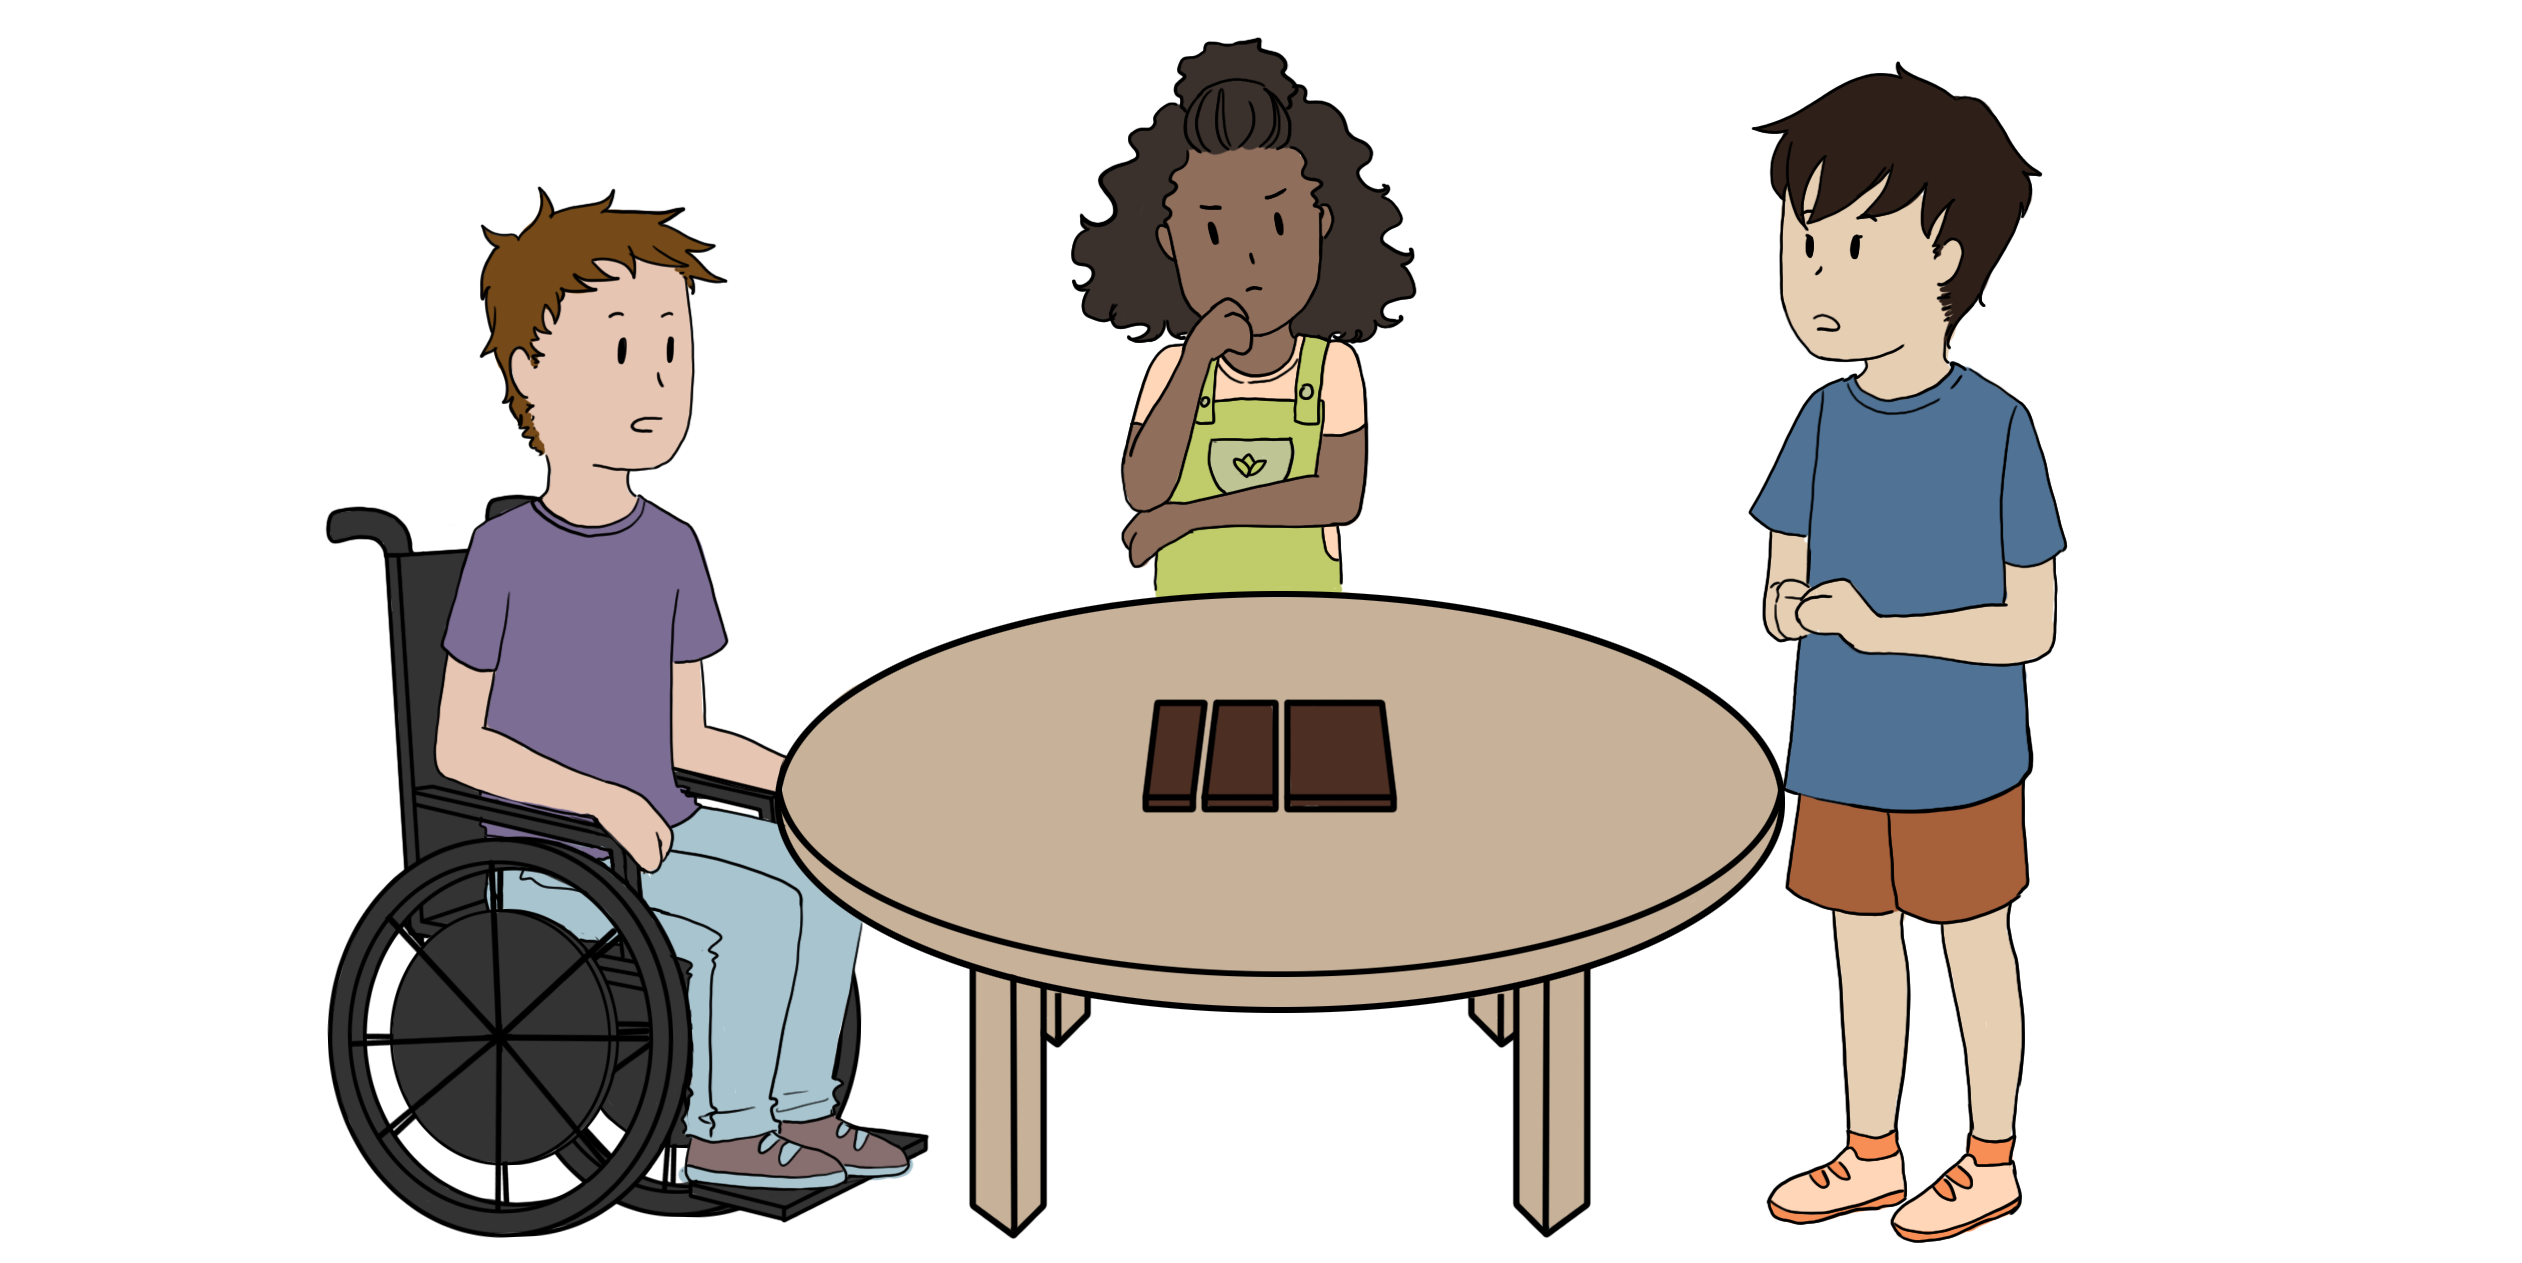
\includegraphics[width=.95\linewidth]{licao01/ativ1_fig01.png}
\end{figure}

\begin{enumerate} %s
  \item Você concorda com essa divisão? Explique.
  \item Com essa divisão, os três amigos receberam a mesma quantidade de chocolate?
  \item Desenhe uma divisão da barra de chocolate que permita que os 3 amigos recebam quantidades iguais de chocolate.

\begin{figure}[H]
\centering

\begin{tikzpicture}
\draw[fill=chocolate, scale=1.25] (0,0) rectangle (4.5,2);        
\end{tikzpicture}
\end{figure}

  \item Considerando a divisão da barra de chocolate em 3 partes iguais, como você nomearia a quantidade de chocolate que cada amigo receberia?
\end{enumerate} %s

\end{atividade}


\begin{atividade}{}\label{chap1-ativ2}
Três pizzas inteiras, de mesmo tamanho, foram repartidas entre as crianças de uma turma. Para isso, a turma foi dividida em três grupos com quatro crianças cada. Veja como cada grupo repartiu a sua pizza.

\begin{figure}[H]
\centering

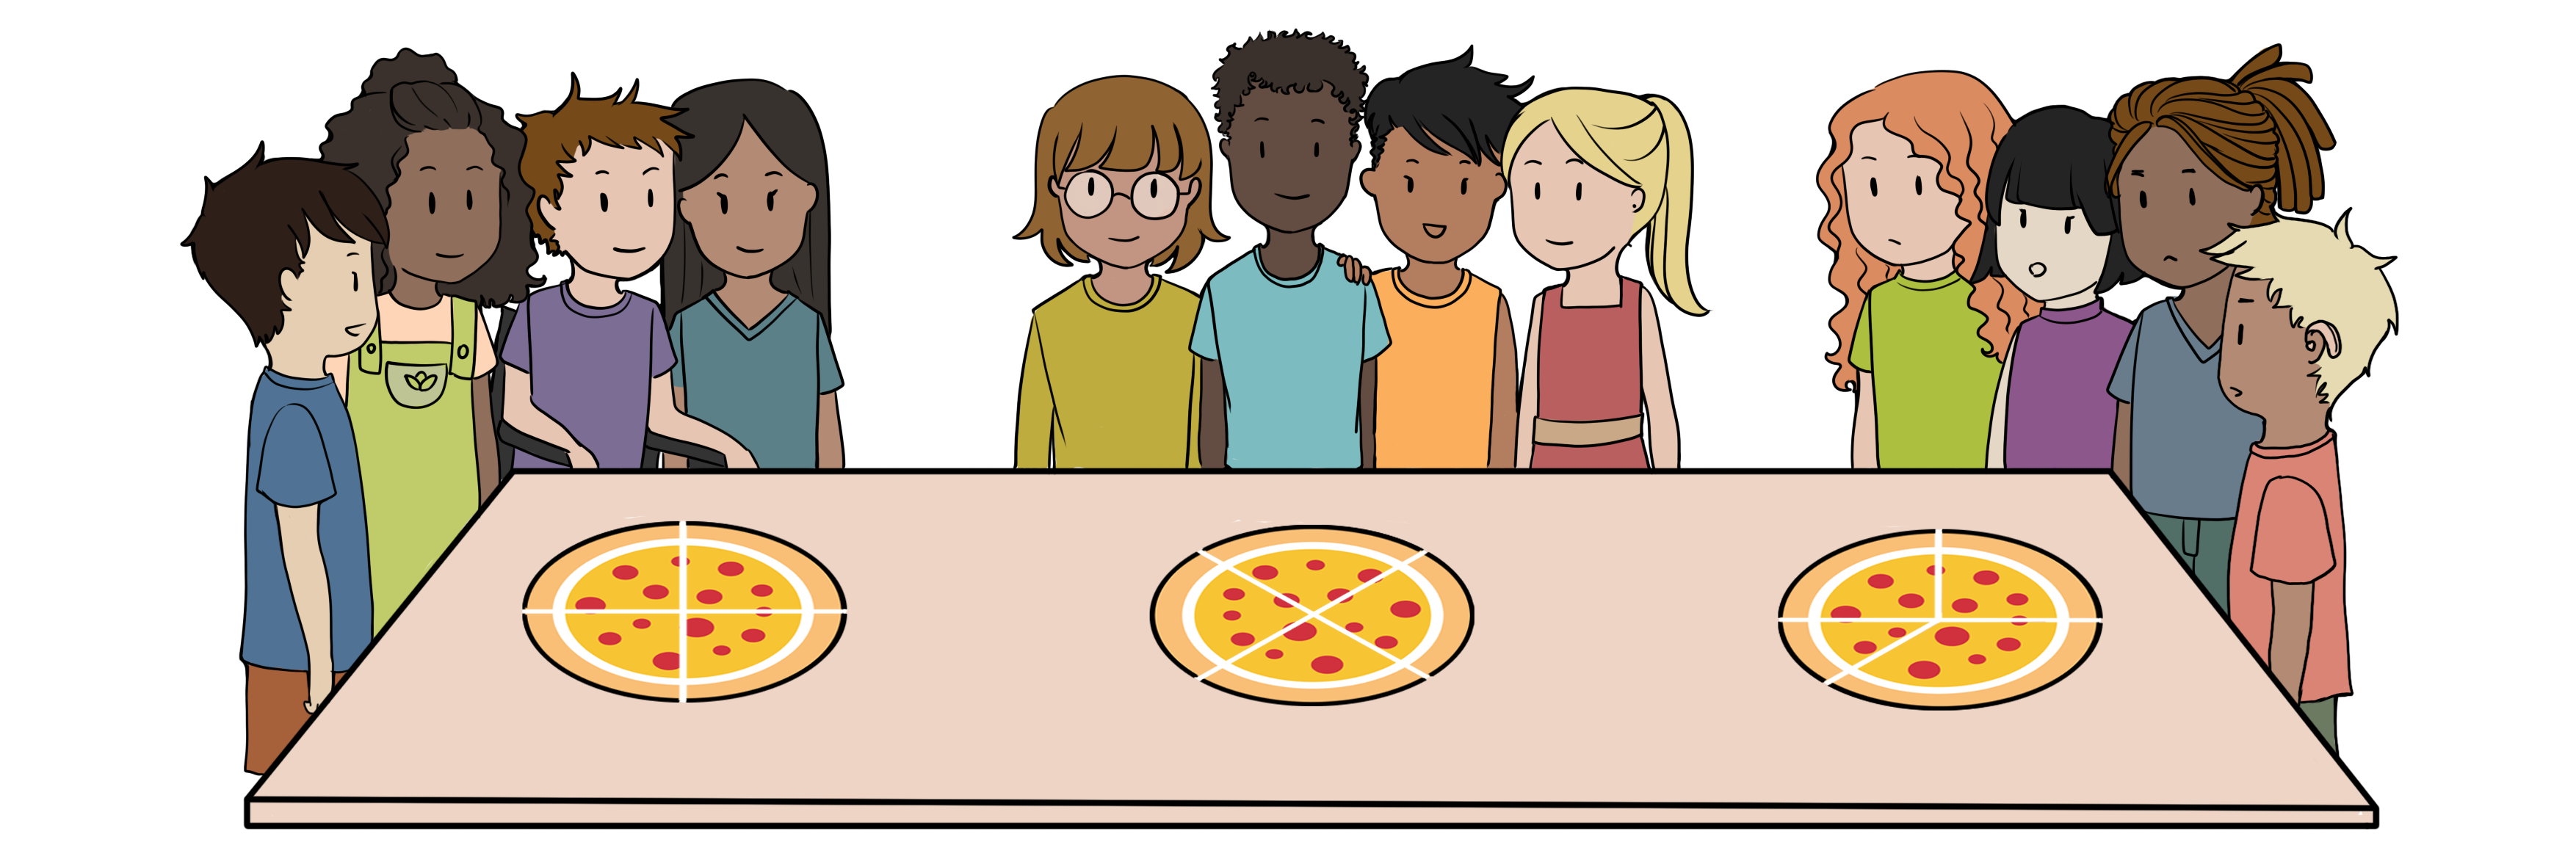
\includegraphics[width=.7\linewidth]{licao01/ativ2_fig01-agnes.png}

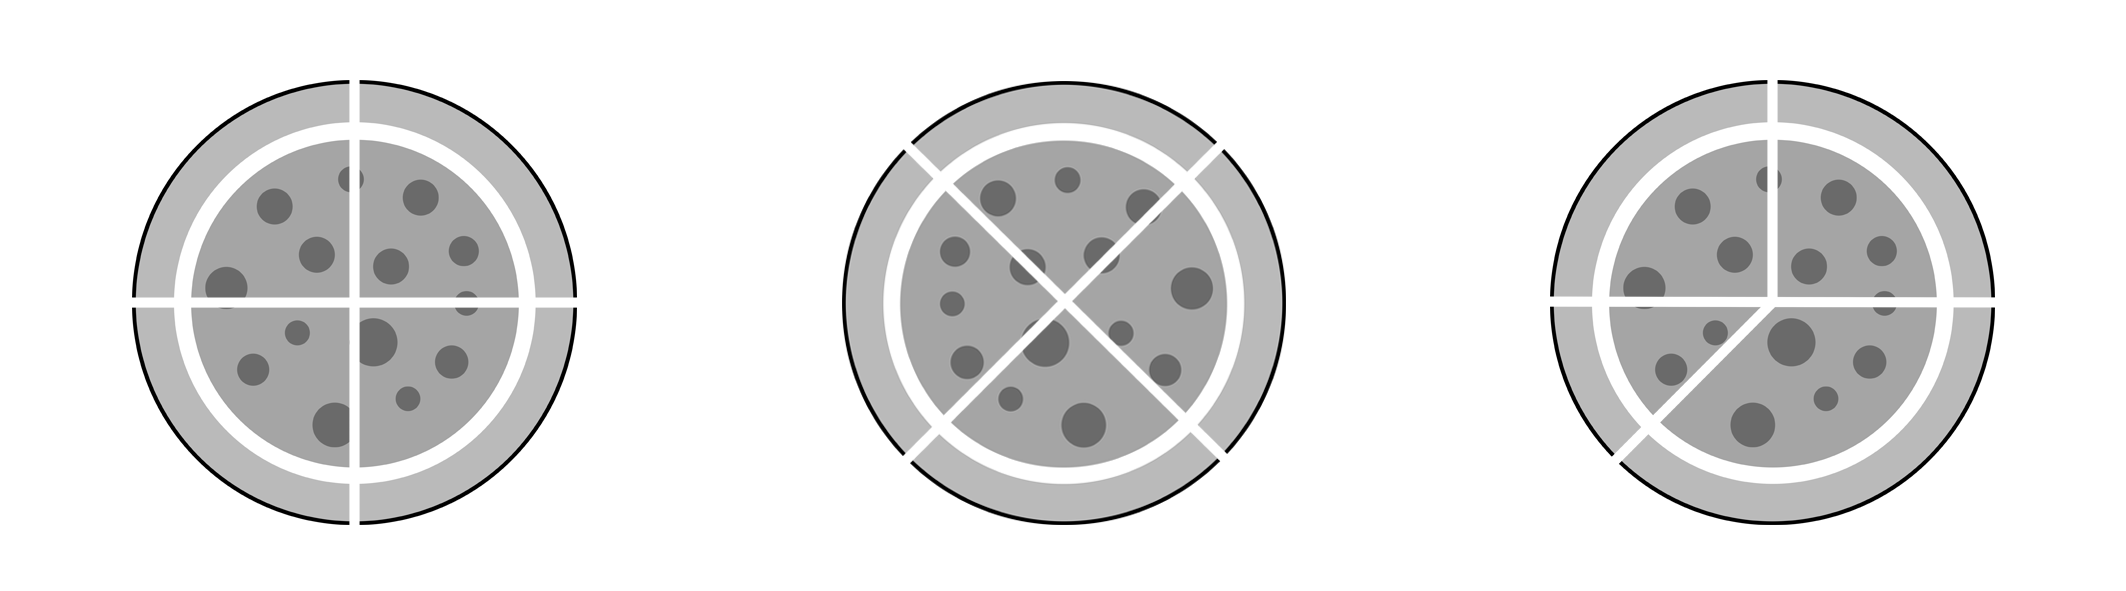
\includegraphics[width=.6\linewidth]{licao01/ativ2_fig02-agnes.png}
\end{figure}

\begin{enumerate} %d
\item Cada um dos três grupos repartiu a sua pizza na mesma \textbf{quantidade de fatias} que os outros grupos?
\item Dessa maneira, todas as crianças da turma receberam a mesma \textbf{quantidade de pizza}?
\item É verdade que em algum dos grupos, as 4 crianças receberam a mesma quantidade de pizza? Se sim, em qual? Considerando a pizza inteira, como você nomearia cada uma das fatias de pizza desse grupo?
\end{enumerate} %d

\end{atividade}

\begin{atividade}{}\label{chap1-ativ3}


Alice quer enfeitar a sala de aula e pretende pendurar os enfeites utilizando pedaços de barbante. Para que os enfeites fiquem todos na mesma altura, quer cortar o barbante em pedaços iguais. Ajude Alice a cortar o barbante (você receberá o barbante do seu professor).


\begin{figure}[H]
\centering

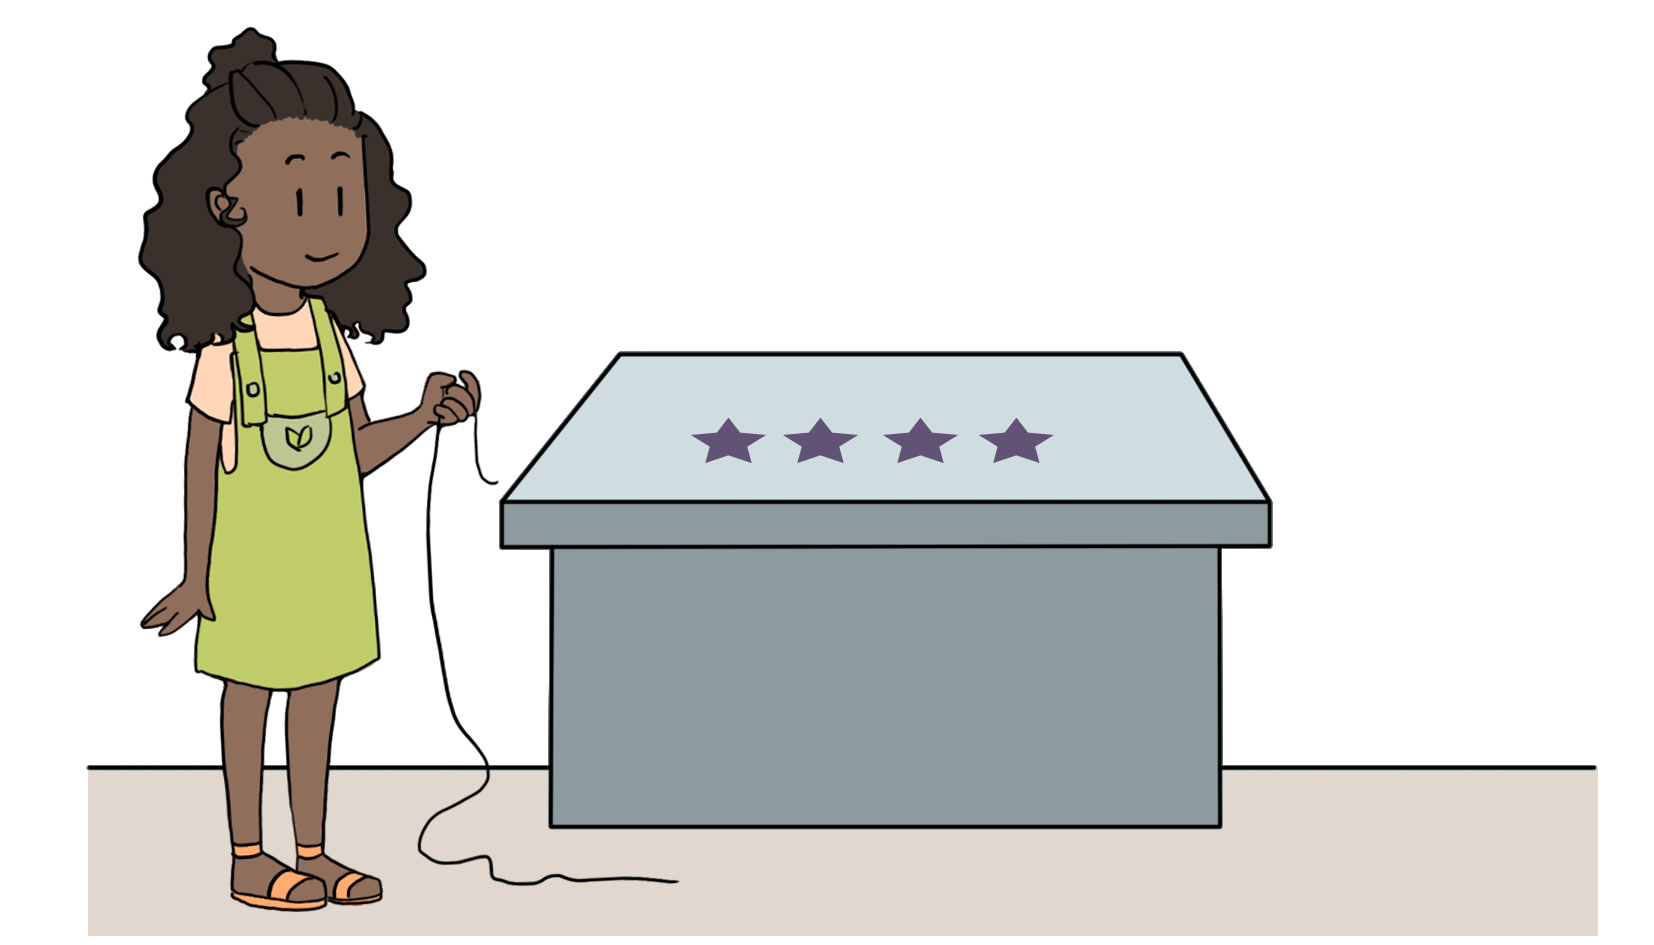
\includegraphics[width=.55\linewidth]{licao01/ativ3_fig01-agnes.png}
\end{figure}


\end{atividade}

\section{Organizando as Ideias}

Nas atividades anteriores, a barra de chocolate, a pizza e o pedaço de barbante foram partidos \textbf{em partes com quantidades iguais}.
Em cada um dos casos, o que foi repartido é chamado \textbf{unidade}. Cada uma das partes em que essas unidades foram repartidas igualmente é uma \textbf{fração da unidade}. Assim, por exemplo, um quarto de uma pizza é uma fração da pizza e a pizza é unidade. Se a unidade for um barbante, um quarto do barbante será uma fração do barbante.


\begin{figure}[H]
\centering

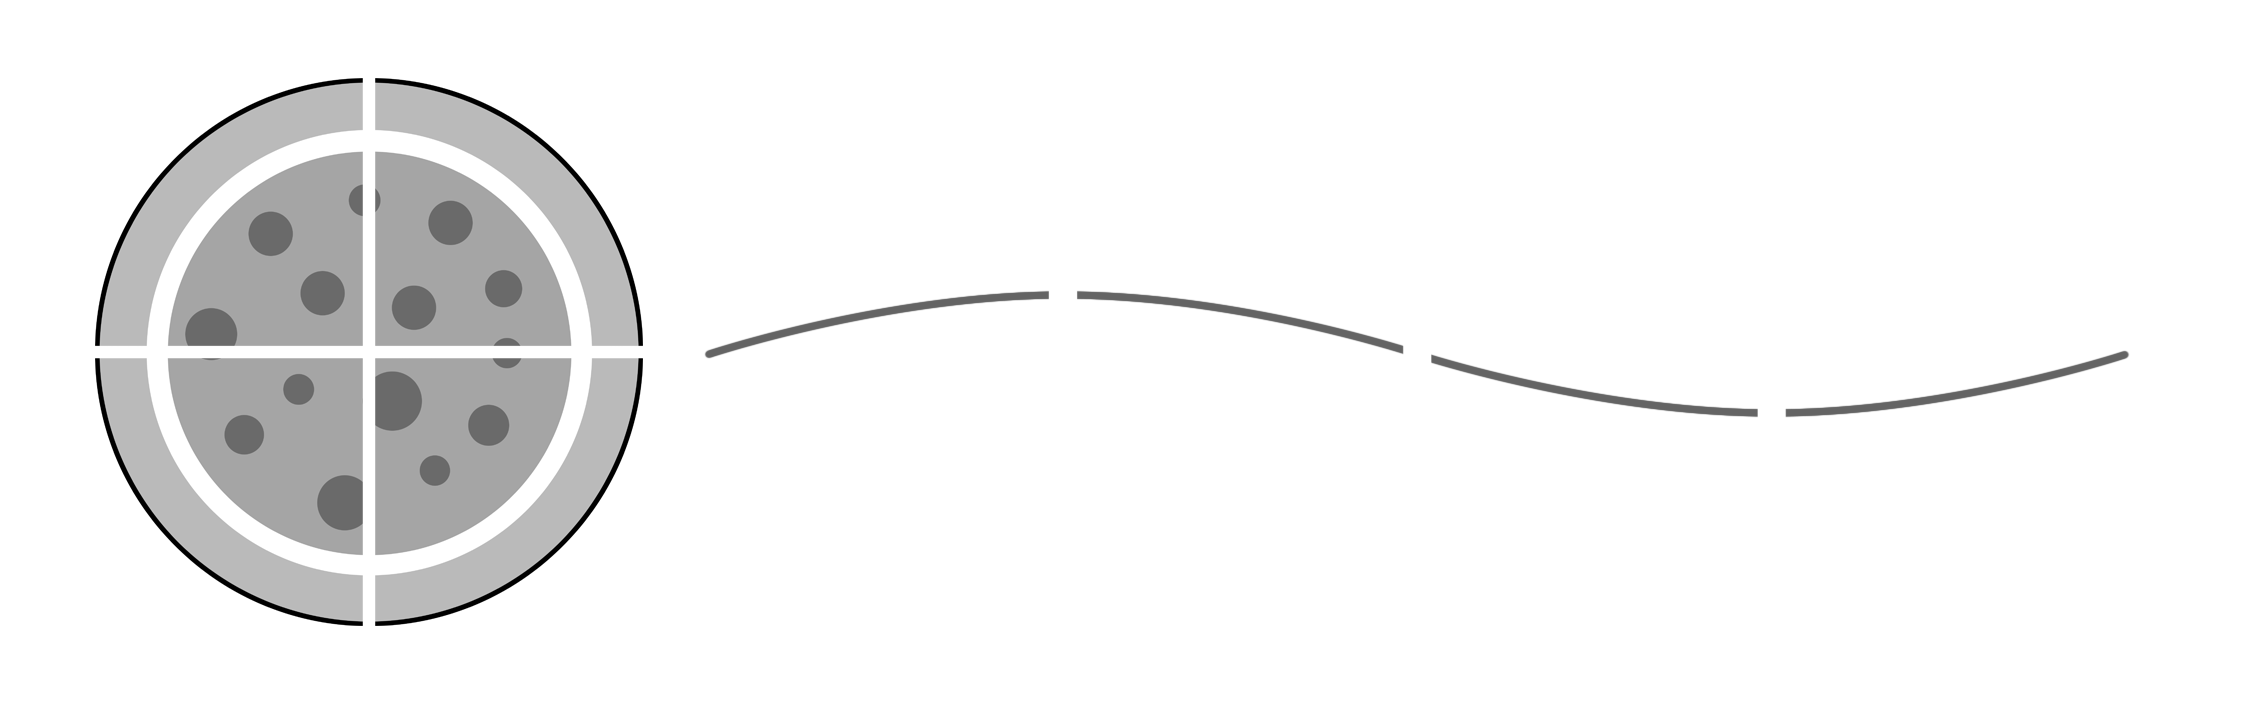
\includegraphics[width=300pt, keepaspectratio]{licao01/orgideias_fig01-agnes.png}
\end{figure}


O nome dado à fração da unidade depende da quantidade de partes em que a unidade é dividida. Ao dividir uma unidade qualquer em duas partes iguais, ou ao meio, cada uma das partes é chamada de \textit{um meio} ou \textit{a metade} da unidade.

Por exemplo, se uma barra de chocolate é repartida igualmente entre dois amigos, a quantidade que caberá a cada um dos amigos é \textit{um meio} da barra de chocolate (ou \textit{metade} da barra). Nesse exemplo, a unidade é a barra de chocolate.


\begin{figure}[H]
\centering

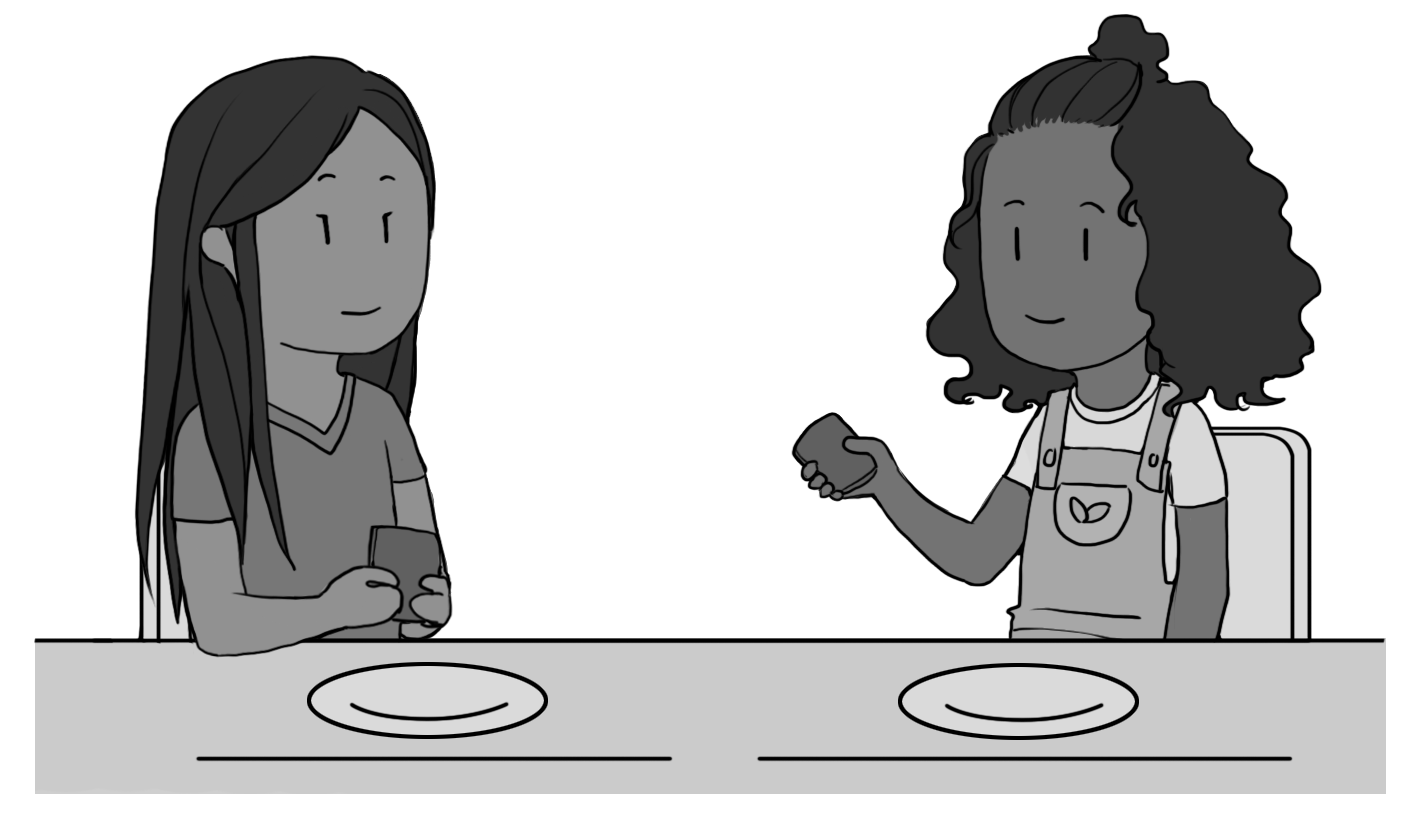
\includegraphics[width=.6\textwidth, keepaspectratio]{licao01/orgideias_fig02-agnes.png}
\end{figure}


Ao dividir uma unidade em três partes iguais, cada uma das partes é chamada de \textit{um terço} ou \textit{a terça parte} da unidade.

Por exemplo, se, para preparar uma receita, é necessário acrescentar \textit{um ter\-ço} de um litro de leite, então para colocar a quantidade correta de leite na receita, é preciso repartir o litro de leite em três partes iguais e usar apenas uma dessas partes. Nesse caso, cada uma das partes é \textit{um terço} do litro de leite. A unidade é um litro de leite.


\begin{figure}[H]
\centering

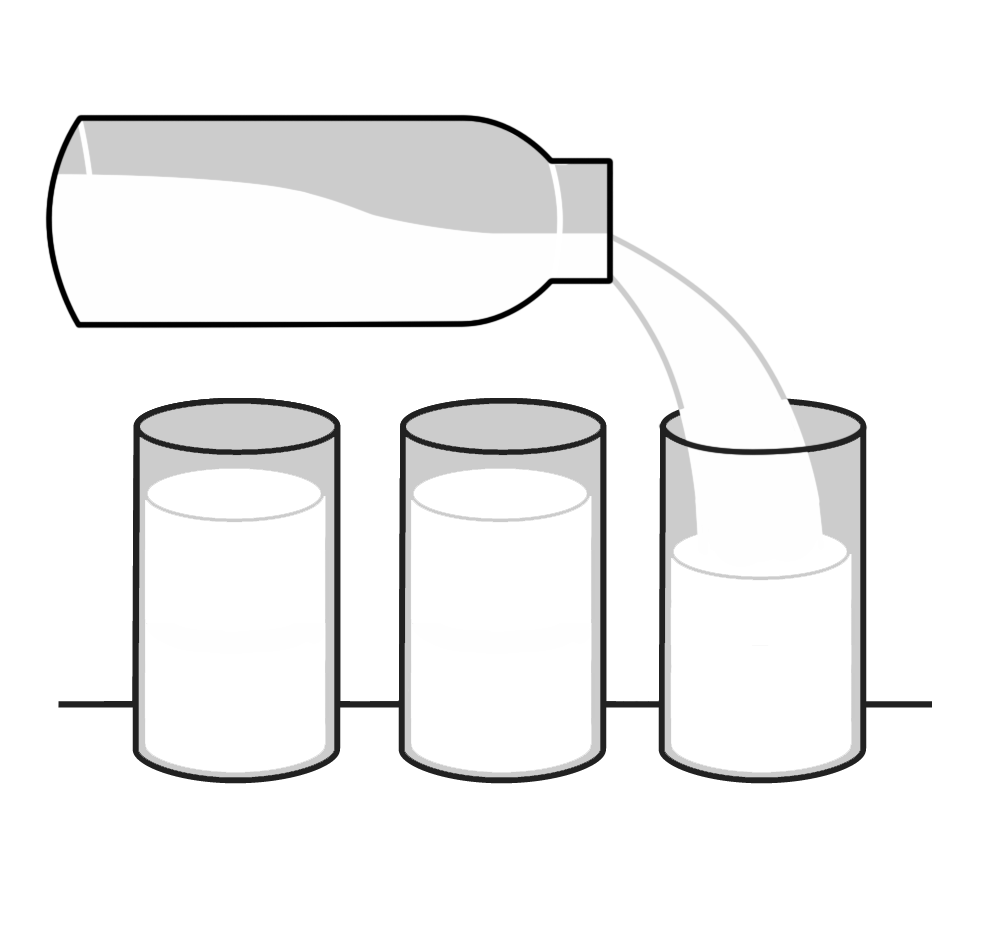
\includegraphics[width=120pt, keepaspectratio]{licao01/copos-incompletos-agnes.png} $\quad$ 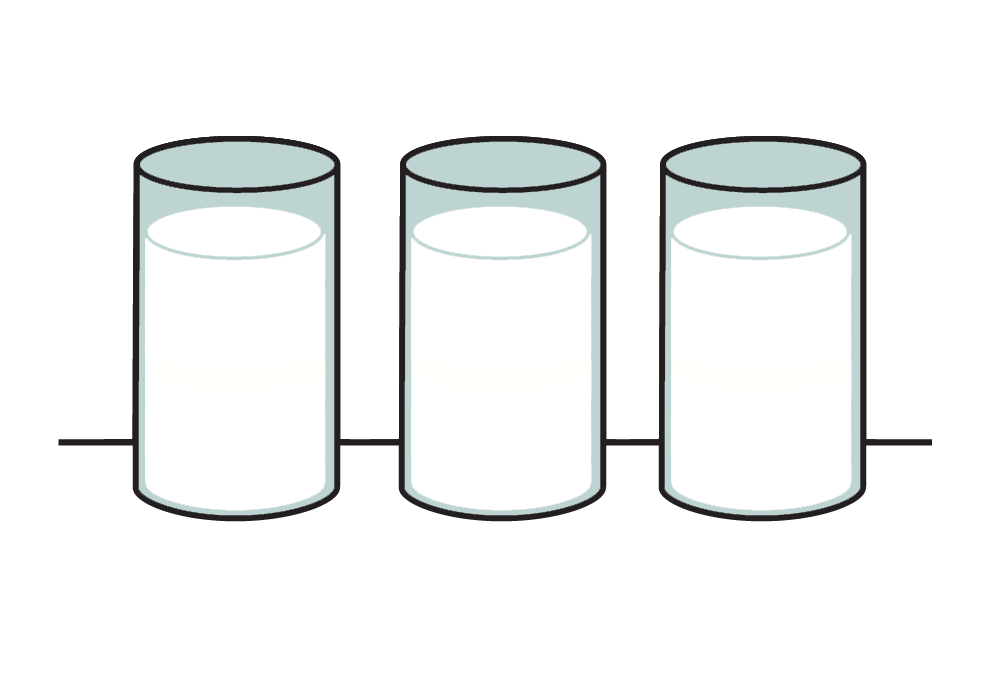
\includegraphics[width=120pt, keepaspectratio]{licao01/copos-cheios-agnes.png}
\end{figure}


Ao dividir uma unidade em quatro partes iguais, cada uma das partes é chamada de \textit{um quarto} ou \textit{quarta parte} da unidade.

Por exemplo, a parte colorida da figura é um quarto da figura. Neste caso, a figura é a unidade.


\begin{figure}[H]
\centering

\begin{tikzpicture}[scale=2.5, every path/.style=very thick]
\fill [cbblue] (0,1) -- (.5,.5) -- (1,1);
\draw (0,0) rectangle (1,1);
\draw (0,0) -- (1,1);
\draw (1,0) -- (0,1);

\end{tikzpicture}
\end{figure}


Da mesma forma, ao dividir uma unidade em cinco partes iguais, cada uma das partes é chamada de \textit{um quinto} ou \textit{quinta parte} da unidade.

Por exemplo, na época do império \textit{um quinto} de todo ouro pesado nas Casas de Fundição no Brasil era pago em impostos à Coroa Portuguesa. Desta forma, a quantidade de ouro pago em impostos à Coroa Portuguesa era igual a \textit{um quinto} ou a \textit{quinta parte} do ouro pesado nas Casas de Fundição no Brasil.


\begin{figure}[H]
\centering

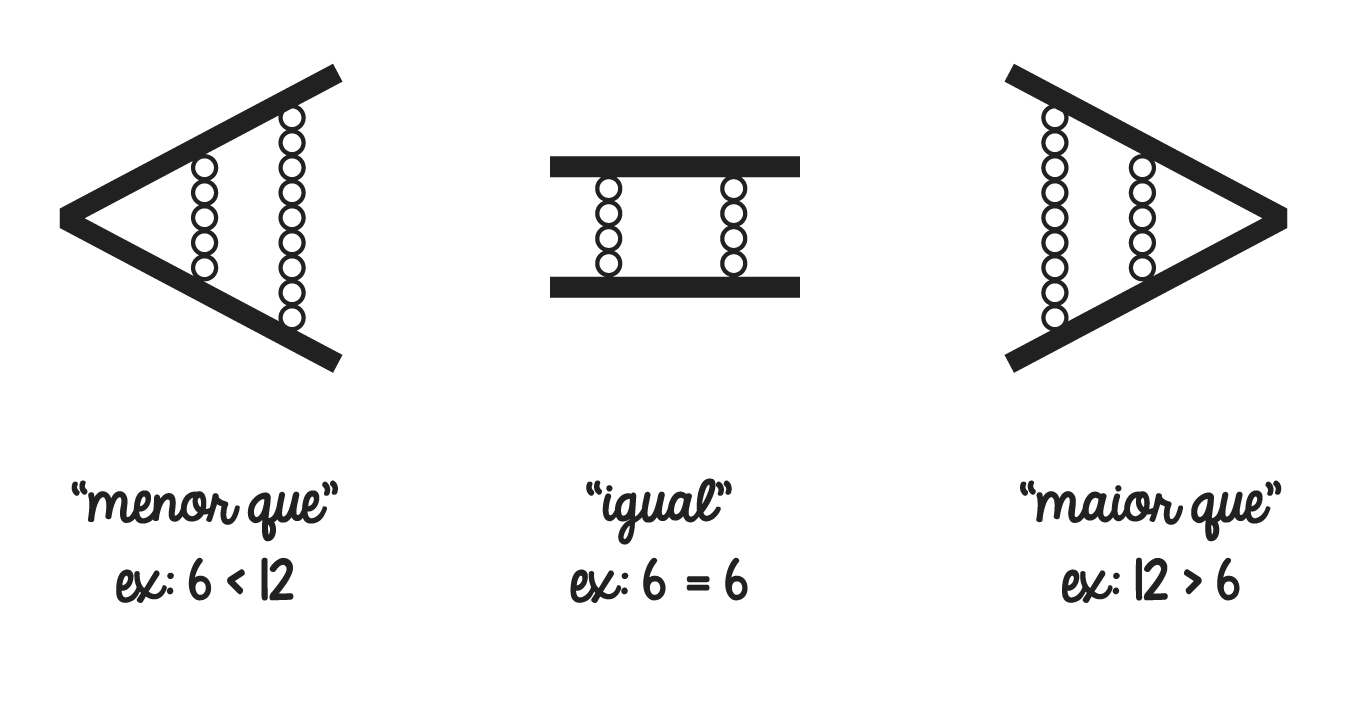
\includegraphics[width=.7\linewidth, keepaspectratio]{licao01/orgideias_fig05.png}
\end{figure}


\section{Mão na Massa}

\begin{atividade}{}\label{chap1-ativ4}

\begin{enumerate} %s
  \item Quais dos oito retângulos a seguir foram partidos em \textit{quartos}? 


\begin{figure}[H]
\centering

\begin{tikzpicture}[every node/.style={scale=.6}, node distance=5cm]
   % primeiro de cima
   % [fill=common, fill opacity=.3]
\node (pink)
  {\begin{tikzpicture}
  \fill[cbpink] (0,0) rectangle (4,6);
    \draw (0,0) rectangle (1,6);
    \draw (1,0) rectangle (2,6);
    \draw (2,0) rectangle (3,6);
    \draw (3,0) rectangle (4,6);
  \end{tikzpicture}};
  
  % segundo de cima
\node [right of=pink] (green)
	{\begin{tikzpicture}
	\draw[fill=stred] (5,0) rectangle (9,3);
	  	\draw[fill=stred] (5,3) rectangle (9,6);
	  	\draw (5,0) -- (9,3);
	  	\draw (5,3) -- (9,6);
	\end{tikzpicture}};

  % terceiro de cima    
\node [right of=green] (brown)
	{\begin{tikzpicture}
	\fill[cbred] (0,0) rectangle (4,6);
	  	\draw(0,0) rectangle (4,1.5);
	  	\draw (0,1.5) rectangle (4,3);
	  	\draw (0,3) rectangle (4,4.5);
	  	\draw (0,4.5) rectangle (4,6);
	\end{tikzpicture}};

  % quarto de cima
\node [right of=brown] (olive)
	{\begin{tikzpicture}
	\fill[cbolive] (5,0) rectangle (9,6);
	  	\draw (5,0) rectangle (9,3);
	  	\draw (5,3) rectangle (9,6);
	  	\draw (7,0) -- (7,6);
	\end{tikzpicture}};

\node [below of=pink, node distance=7cm] (purple)
  {\begin{tikzpicture}
  \fill[cbpurple] (10,0) rectangle (14,6);  
      \draw (10,0) rectangle (14,3);
      \draw (10,3) rectangle (14,6);
      \draw (12,0) -- (12,3);
      \draw (10,4.5) -- (14,4.5);
  \end{tikzpicture}};
  
  % 2 debaixo
  %\draw (15,0) rectangle (19,6);
\node [right of=purple] (yellow)
  {\begin{tikzpicture}
    \filldraw[fill=cbyellow] (15,0) rectangle (19,3);
      \filldraw[fill=cbyellow] (15,3) rectangle (19,6);
      \draw (15,1.5) -- (19,1.5);
     \draw (15,3) -- (19,6);
    \end{tikzpicture}};

  % 3 debaixo
\node [right of=yellow] (gray)
  {\begin{tikzpicture}
  \fill[cbgray, opacity=.8] (10,0) rectangle (14,6);
      \draw[fill=cbgray, fill opacity=.3] (10,0) rectangle (14,3);
      \draw[fill=cbgray, fill opacity=.3] (10,3) rectangle (14,6);
      \draw (12,0) -- (12,3);
      \draw (10,6) -- (14,3);
  \end{tikzpicture}};

  % 4 debaixo  
\node [right of=gray] (orange)
  {\begin{tikzpicture}
  \fill[cborange] (0,0) rectangle (4,6);
      \draw[fill=cborange, fill opacity=.3] (0,0) rectangle (4,6);
      \draw (1,0) -- (1,6);
      \draw (2,0) -- (2,6);
      \draw (2,3) -- (4,3);
  \end{tikzpicture}};

\end{tikzpicture}
\end{figure}


  \item     Desenhe um retângulo e faça uma partição desse retângulo em ~quatro partes que não sejam todas quartos.
\end{enumerate}
\end{atividade}

\begin{refletindo*}{}{}
  Na atividade anterior, as partes em que os retângulos foram divididos são quartos dos retângulos, mesmo tendo formas diferentes.


\begin{figure}[H]
\centering

    \begin{tikzpicture}[scale=.6]
    \draw[fill=common] (10,0) rectangle (14,3);
  \draw[fill=common] (10,3) rectangle (14,6);
  \draw (12,0) -- (12,3);
  \draw (10,6) -- (14,3);
    \end{tikzpicture}
\end{figure}


  Se uma unidade é repartida em partes com quantidades iguais, essas partes são frações dessa unidade mesmo que tenham formas diferentes. Observe, nos quadrinhos a seguir, como a pizza foi dividida entre os dois amigos:


\begin{figure}[H]
\centering

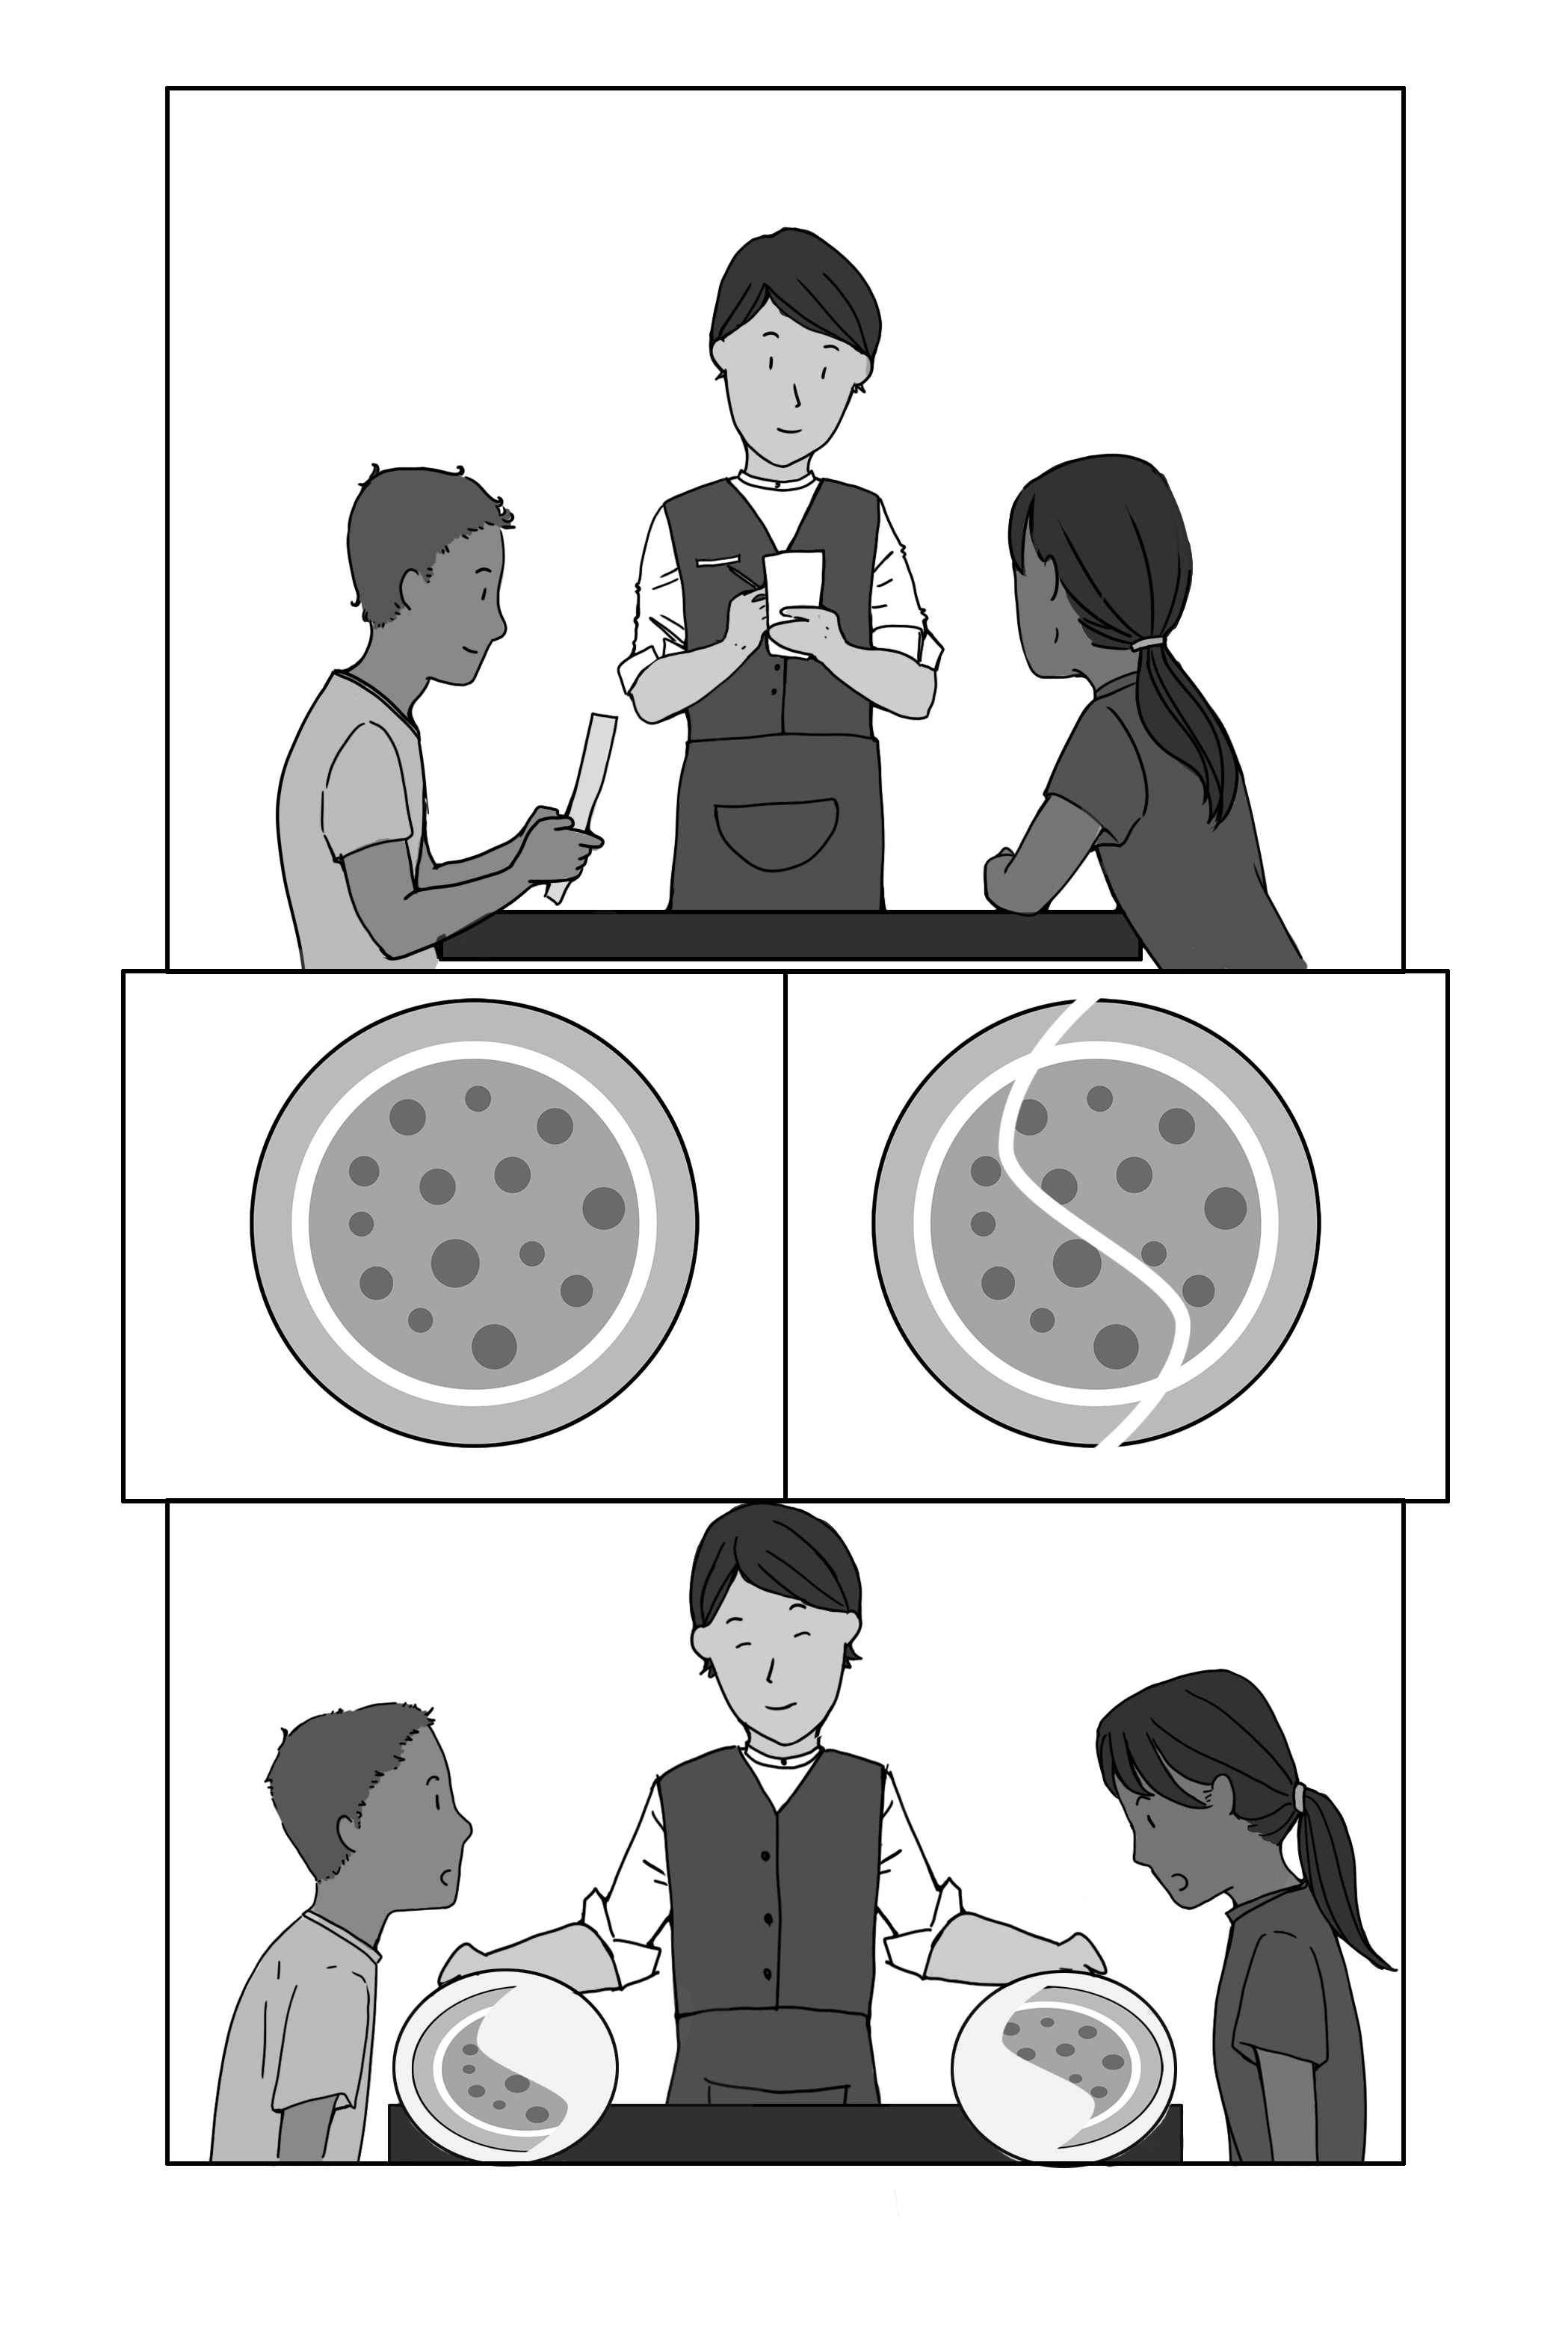
\includegraphics[width=.6\textwidth, keepaspectratio]{licao01/pizzaria-do-artista-agnes}

\end{figure}

\end{refletindo*}

\begin{atividade}{}\label{chap1-ativ5}

\begin{enumerate}
\item O triângulo menor é um terço de uma das figuras. Qual é essa figura? Explique. 
\item O triângulo menor é um quarto de alguma dessas figuras? Qual ou quais?
\item Agora é a sua vez: desenhe uma unidade da qual o triângulo menor seja um quinto.  
\item Que fração o triângulo menor é da segunda figura na terceira linha?
\item Desafio: Que fração o triângulo menor é do retângulo? 
\end{enumerate}

% \begin{table}[H]
% \centering

% \begin{tabular}{ccc}
% \begin{tikzpicture}[scale=2]
% \fill [cbgray] (60:0) -- (120:1) -- (180:1) -- cycle;
% \end{tikzpicture}
%   &
% %losango
% \begin{tikzpicture}[scale=2,rotate=90]
% \fill [cbpink] (60:0) -- (120:1) -- (180:1) -- ++(300:1) -- cycle;
% \end{tikzpicture}
%   &
% %estrela de  seis pontas
% \begin{tikzpicture}[scale=2]
% \fill [cbpurple] (0,0) -- (60:1) -- (120:1) -- cycle;
% \fill [cbpurple,shift={(.5,1.71/6)}] (60:0) -- (120:1) -- (180:1) -- cycle;
% \end{tikzpicture}
%     \\
% \end{tabular}
% \end{table}
\renewcommand{\arraystretch}{2.5}
\begin{longtable}[c]{ccc}
\endfirsthead
\begin{tikzpicture}[scale=2]
\fill [cbgray] (60:0) -- (120:1) -- (180:1) -- cycle;
\end{tikzpicture}
  &
%losango
\begin{tikzpicture}[scale=2,rotate=90]
\fill [cbred] (60:0) -- (120:1) -- (180:1) -- ++(300:1) -- cycle;
\end{tikzpicture}
  &
%estrela de  seis pontas
\begin{tikzpicture}[scale=2]
\fill [cbpurple] (0,0) -- (60:1) -- (120:1) -- cycle;
\fill [cbpurple,shift={(.5,1.71/6)}] (60:0) -- (120:1) -- (180:1) -- cycle;
\end{tikzpicture}
    \\
%paralelogramo
\begin{tikzpicture}[scale=2]
\fill [stred]  (120:1) -- ++(180:1) -- ++(240:1) -- ++(360:2) -- ++(60:1) -- cycle;
\end{tikzpicture}
  &
%retângulo
\begin{tikzpicture}[scale=2]
\fill [cborange] (0,0) -- (1,0) -- (1,1.732/2) -- (0,1.732/2) -- cycle;
\end{tikzpicture}
  &
    %trapézio:
\begin{tikzpicture}[scale=2]
\fill [cbpink] (60:0) -- (120:1) -- ++(180:1) -- +(240:1) -- cycle;
\end{tikzpicture}
  \\
  %hexágono
\begin{tikzpicture}[scale=2]
\fill [cbolive] (60:0) -- (120:1) -- ++(180:1) -- ++(240:1) -- ++(300:1) -- ++(360:1) -- cycle;
\end{tikzpicture}
&
%Bandeirinha
\begin{tikzpicture}[scale=2,xscale=-1]
\filldraw [cbyellow]  (120:1) -- ++(180:1) -- ++(240:1) -- ++(360:2) -- ++(60:1) -- cycle;
\filldraw [cbyellow,yscale=-1]  (120:1) -- ++(180:1) -- ++(240:1) -- ++(360:2) -- ++(60:1) -- cycle;
\end{tikzpicture}
&
%Triângulo ampliado
\begin{tikzpicture}[scale=4]
\fill [lightred] (60:0) -- (120:1) -- (180:1) -- cycle;
\end{tikzpicture}
\end{longtable}

\end{atividade}

\begin{atividade}{}\label{chap1-ativ6}

Em cinco das figuras a seguir, a parte em destaque é um terço da figura. Identifique essas figuras.

\begin{tasks}(2)
\task \adjustbox{valign=t}
{
\resizebox{.4\linewidth}{!}
{
  \begin{tikzpicture}
    \draw[ultra thick, attention, mono color=attention!70!black] (90:2 cm)  -- (210:2 cm);
    \draw[ultra thick, attention, mono color=attention!70!black] (330:2 cm) -- (90:2 cm);
    \draw[very thick, common] (210:2 cm)  -- (330:2 cm);
  \end{tikzpicture}
}
}

\task \adjustbox{valign=t}
{
\resizebox{.4\linewidth}{!}
{
\begin{tikzpicture}
  \draw[very thick, common] (90:2 cm)  -- (210:2 cm);
  \draw[ultra thick, attention, mono color=attention!70!black] (210:2 cm)  -- (330:2 cm);
  \draw[very thick, common] (330:2 cm) -- (90:2 cm);
\end{tikzpicture}
}
}

\task \adjustbox{valign=t}
{
\resizebox{.7\linewidth}{!}
{
\begin{tikzpicture}
  \draw[very thick, common] (0,3) -- (3,0);
  \draw[ultra thick, attention, mono color=attention!70!black] (3,0) -- (6,3);
  \draw[very thick, common] (6,3) -- (9,0);
\end{tikzpicture}
}
}

\task \adjustbox{valign=t}
{
\resizebox{.7\linewidth}{!}
{
  \begin{tikzpicture}
    \draw[ultra thick, attention, mono color=attention!70!black] (0,3) -- (3,0);
    \draw[ultra thick, attention, mono color=attention!70!black] (3,0) -- (6,3);
    \draw[very thick, common] (6,3) -- (9,0);
  \end{tikzpicture}
}
}

\task \adjustbox{valign=t}
{
\resizebox{.7\linewidth}{!}
{
\begin{tikzpicture}[scale=3]
    \draw[fill=common, fill opacity=.3] (0,0) rectangle (3,1);
    \draw[fill=attention] (3,0) rectangle (6,1);
    \draw[fill=common, fill opacity=.3] (6,0) rectangle (9,1);
\end{tikzpicture}
}
}

\task \adjustbox{valign=t}
{
\resizebox{.7\linewidth}{!}
{
\begin{tikzpicture}[scale=3]
    \draw[fill=common, fill opacity=.3] (0,0) rectangle (2,1);
    \draw[fill=attention] (2,0) rectangle (6,1);
    \draw[fill=common, fill opacity=.3] (6,0) rectangle (9,1);
\end{tikzpicture}
}
}

\task \adjustbox{valign=t}
{
\resizebox{.4\linewidth}{!}
{
\begin{tikzpicture}[scale=0.7]

\filldraw [fill=common, fill opacity=.3, draw=black] (0:2 cm) -- (90:2 cm) -- (180:2 cm) -- (0,0) -- ( (270:2 cm) --cycle;
\fill[attention] (180:2 cm) -- (270:2cm) -- (0,0) -- cycle;
\draw (180:2 cm) -- (0:2 cm);
\draw (90:2 cm) -- (270:2 cm);
\draw (180:2 cm) -- (270:2 cm);
\end{tikzpicture}
}
}

\task \adjustbox{valign=t}
{
\resizebox{.4\linewidth}{!}
{
\begin{tikzpicture}[scale=0.7]
  \filldraw[fill=attention, draw=black] (-2 cm, 0) -- (0,0) -- (0, 2 cm) arc (90:180:2 cm) -- cycle;
  \filldraw[fill=common, draw=black, fill opacity=.3] (-2 cm, 0) -- (2 cm,0) arc (0:-180: 2cm);
  \fill (0,0) circle (2 pt);
\end{tikzpicture}
}
}

\task \adjustbox{valign=t}
{
\resizebox{.5\linewidth}{!}
{
\begin{tikzpicture}[scale=6]
  \filldraw[fill=common, fill opacity=.3, draw=black] (0,0) -- (0.5,0.5) -- (4,0.5) -- (4,2) -- (4.5,2.5) -- (4.5,0)--cycle;
  \fill[attention] (0,0) -- (0.5,0.5) -- (0.5,2) -- (4,2) -- (4.5,2.5) -- (0,2.5)--cycle;
 \draw (0,0) rectangle (4.5,2.5);
  \draw (0.5,0.5) rectangle (4,2);
\end{tikzpicture}
}
}

\task \adjustbox{valign=t}
{
\resizebox{.6\linewidth}{!}
{
  \begin{tikzpicture}[x=1mm, y=1mm]%[scale=60]
  \tikzset{
  annotated cuboid/.pic={
    \tikzset{%
      every edge quotes/.append style={midway, auto},
      /cuboid/.cd,
      #1
    }
    \draw [every edge/.append style={pic actions, densely dashed, opacity=0}, pic actions]
    (0,0,0) coordinate (o) -- ++(-\cubescale*\cubex,0,0) coordinate (a) -- ++(0,-\cubescale*\cubey,0) coordinate (b) edge coordinate [pos=1] (g) ++(0,0,-\cubescale*\cubez)  -- ++(\cubescale*\cubex,0,0) coordinate (c) -- cycle
    (o) -- ++(0,0,-\cubescale*\cubez) coordinate (d) -- ++(0,-\cubescale*\cubey,0) coordinate (e) edge (g) -- (c) -- cycle
    (o) -- (a) -- ++(0,0,-\cubescale*\cubez) coordinate (f) edge (g) -- (d) -- cycle;
 },
  /cuboid/.search also={/tikz},
  /cuboid/.cd,
  width/.store in=\cubex,
  height/.store in=\cubey,
  depth/.store in=\cubez,
  units/.store in=\cubeunits,
  scale/.store in=\cubescale,
  width=100,
  height=100,
  depth=100,
  units=cm,
  scale=.1,
}

    \pic [fill=attention] at (50,0) {annotated cuboid={width=100, height=100, depth=14}};
    \pic [fill=common, fill opacity=.3] at (70,0) {annotated cuboid={width=200, height=100, depth=14}};
    \draw [dashed, lightgray] (50,-10,-1.4) -- (70,-10,-1.4);
    \draw [dashed, lightgray] (60,-10,0) -- (60,-10,-1.4) -- (60,0,-1.4);
    \draw [dashed] (60,0,-1.4) -- (60,0,0) -- (60,-10,0);
    \end{tikzpicture}
}
}
\end{tasks}


\end{atividade}

\begin{atividade}{}\label{chap1-ativ7}
\tikzset{x=1mm,y=1mm}


\begin{enumerate}
\item Na tabela a seguir, a primeira coluna mostra uma figura que é uma fração de uma unidade. Na segunda, o nome que usamos para essa fração. Desenhe uma unidade na terceira coluna, unindo frações como essa.
  
  \def\h{1.4}
  
\begin{center}
\begin{tabular}{|m{0.275\linewidth}|c|p{.25\linewidth}|}
\hline
\centering Fração da unidade & \centering Nome da fração da unidade  & \centering Unidade\tabularnewline
\hline 
\centering \begin{tikzpicture}[scale=2]
\draw [fill=common, fill opacity=.3] (0,0) arc (0:90:3) -- (-3,0) -- cycle;
\end{tikzpicture}
&\centering \parbox[c][\h cm][c]{0.01cm}{  } metade  &  \\
\hline
\end{tabular}
\end{center}

\item A seguir, complete cada linha da tabela como no item anterior.

\centering
\begin{longtable}{|m{0.275\linewidth}|c|p{.25\linewidth}|}
\hline
\endfirsthead
\centering Fração da unidade & \centering Nome da fração da unidade  & \centering Unidade \tabularnewline
\hline
\centering \begin{tikzpicture}[scale=2]
\draw [fill=common, fill opacity=.3] (0,0) arc (0:90:3) -- (-3,0) -- cycle;
\end{tikzpicture}
&\centering \parbox[c][\h cm][c]{0.01cm}{  } metade  &  \\
\hline
\centering\begin{tikzpicture}[scale=2]
\draw [fill=common, fill opacity=.3] (0,0) arc (0:90:3) -- (-3,0) -- cycle;
\end{tikzpicture}        &\parbox[c][\h cm][c]{0.01cm}{  } \centering   um terço  &  \\
\hline
\centering \begin{tikzpicture}[scale=2]
\draw [fill=common, fill opacity=.3] (0,0) arc (0:90:3) -- (-3,0) -- cycle;
\end{tikzpicture}        & \centering \parbox[c][\h cm][c]{0.01cm}{  } um quarto  &  \\
\hline
\centering \begin{tikzpicture}[scale=2]
\draw [fill=common, fill opacity=.3] (0,0) rectangle (3,3);
\end{tikzpicture}
& \centering \parbox[c][\h cm][c]{0.01cm}{  } metade  &  \\
\hline
\centering \begin{tikzpicture}[scale=2]
\draw [fill=common, fill opacity=.3] (0,0) rectangle (3,3);
\end{tikzpicture}
& \centering \parbox[c][\h cm][c]{0.01cm}{  } um terço  &  \\
\hline
\centering \begin{tikzpicture}[scale=2]
\draw [fill=common, fill opacity=.3] (0,0) rectangle (3,3);
\end{tikzpicture}
& \centering \parbox[c][\h cm][c]{0.01cm}{  } um quarto  &  \\
\hline
\centering \begin{tikzpicture}[scale=2]
\draw  (0,0) -- (3,3);
\end{tikzpicture}
& \centering \parbox[c][\h cm][c]{0.01cm}{  } metade  &  \\
\hline
\centering \begin{tikzpicture}[scale=2]
\draw  (0,0) -- (3,3);
\end{tikzpicture}
& \centering \parbox[c][\h cm][c]{0.01cm}{  } um terço  &  \\
\hline
\centering \begin{tikzpicture}[scale=2]
\draw  (0,0) -- (3,3);
\end{tikzpicture}
& \centering \parbox[c][\h cm][c]{0.01cm}{  } um quarto  &  \\
\hline
\centering \begin{tikzpicture}[scale=2]
\draw [fill=common, fill opacity=.3] (90:2) -- (210:2) -- (330:2) -- cycle;
\end{tikzpicture}  & \centering \parbox[c][\h cm][c]{0.01cm}{  } metade  &  \\
\hline
\centering \begin{tikzpicture}[scale=2]
\draw [fill=common, fill opacity=.3] (90:2) -- (210:2) -- (330:2) -- cycle;
\end{tikzpicture}  & \centering \parbox[c][\h cm][c]{0.01cm}{  } um terço  &  \\
\hline
\centering \begin{tikzpicture}[scale=2]
\draw [fill=common, fill opacity=.3] (90:2) -- (210:2) -- (330:2) -- cycle;
\end{tikzpicture}  & \centering \parbox[c][\h cm][c]{0.01cm}{  } um quarto  &  \\
\hline
\end{longtable}


\end{enumerate}

\end{atividade}

\begin{atividade}{}\label{chap1-ativ8}

\begin{enumerate} %s
\item Pinte metade do quadrado a seguir.
\begin{figure}[H]
\centering

\begin{tikzpicture}[x=1mm,y=1mm, scale=.7]  \draw[fill=common, fill opacity=.3] (0,0) rectangle (20,20);  
\end{tikzpicture}
\end{figure}

\item Pinte um quarto do quadrado a seguir.
\begin{figure}[H]
\centering

\begin{tikzpicture}[x=1mm,y=1mm, scale=.7]  \draw[fill=common, fill opacity=.3] (0,0) rectangle (20,20);  
\end{tikzpicture}
\end{figure}

\item Pinte um oitavo do quadrado a seguir.
\begin{figure}[H]
\centering

\begin{tikzpicture}[x=1mm,y=1mm, scale=.7]  \draw[fill=common, fill opacity=.3] (0,0) rectangle (20,20);  
\end{tikzpicture}
\end{figure}
\item Qual é a maior das frações do quadrado: metade, quarto ou oitavo?
\end{enumerate} %s
\end{atividade}


\begin{atividade}{}\label{chap1-ativ9}

\begin{enumerate}  %d
  \item     Pinte metade da figura.
\begin{center}
  \begin{tikzpicture}[x=1cm,y=1cm, scale=0.5]
  \draw[fill=common, fill opacity=.3] (3.,5.) -- (3.,3.) -- (4.7,2.) -- (6.46,3.) -- (8.2,2.) -- (9.9,3.) -- (9.9,5.) -- (8.2,6.)       -- (6.46,5.) -- (4.73,6.) -- cycle;
  \end{tikzpicture}
\end{center}

  \item     Pinte metade da figura de forma diferente da do item anterior.
\begin{center}
  \begin{tikzpicture}[x=1cm,y=1cm, scale=0.5]
  \draw[fill=common, fill opacity=.3] (3.,5.) -- (3.,3.) -- (4.7,2.) -- (6.46,3.) -- (8.2,2.) -- (9.9,3.) -- (9.9,5.) -- (8.2,6.)       -- (6.46,5.) -- (4.73,6.) -- cycle;
  \end{tikzpicture}
\end{center}

  \item     Pinte a metade da figura de forma diferente das dos dois itens anteriores.
\begin{center}
  \begin{tikzpicture}[x=1cm,y=1cm, scale=0.5]
  \draw[fill=common, fill opacity=.3] (3.,5.) -- (3.,3.) -- (4.7,2.) -- (6.46,3.) -- (8.2,2.) -- (9.9,3.) -- (9.9,5.) -- (8.2,6.)       -- (6.46,5.) -- (4.73,6.) -- cycle;
  \end{tikzpicture}
\end{center}


\end{enumerate} %d
\end{atividade}

\begin{atividade}{}\label{chap1-ativ10}


Identifique as figuras em que a parte em destaque é a metade da figura.

\begin{center}
  \begin{tabular}{ccccc}
%retângulos

\begin{tikzpicture}[scale=.5]
 \draw[fill=attention] (0,0) rectangle (3,2);
 \draw[fill=common, fill opacity=.3] (3,0) rectangle (6,2);
 \node at (3,-1) {Figura 1};
\end{tikzpicture}
&
\quad \quad \quad
&
\begin{tikzpicture}[scale=.5]
 \draw[fill=common, fill opacity=.3] (0,0) rectangle (3,2);
 \draw (1,0) -- (1,2);
 \draw (1.5,0) -- (1.5,2);
 \draw (2.2,0) -- (2.2,2);
 \draw[fill=attention] (3,0) rectangle (6,2);
 \node at (3,-1) {Figura 2};
\end{tikzpicture}
&
\quad \quad \quad
&

\begin{tikzpicture}[scale=.5]
 \draw[fill=common, fill opacity=.3] (0,0) rectangle (3,2);
 \draw[fill=common, fill opacity=.3] (3,0) rectangle (6,2);
 \node at (3,-1) {Figura 3};
 \filldraw[fill=attention, draw=black] (0,2) rectangle (6,1.2);
 \end{tikzpicture}
\\
 % círculos

\begin{tikzpicture}[scale=.5]
  \filldraw[fill=attention, draw=black] (0,-2) arc (-90:90: 2);
  \draw (0, 2) -- (0, -2);
  \draw[fill=common, fill opacity=.3] (0,2) arc (90:270:2);
  \node at (0,-3) {Figura 4};
\end{tikzpicture}
&&

\begin{tikzpicture}[scale=.5]
 \filldraw[fill=attention, draw=black] (45:2) arc (45:225:2);
 \draw[fill=common, fill opacity=.3] (225:2) arc (225:405:2);
 \node at (0,-3) {Figura 5};
 \draw (0,0) -- (0,-2);
 \draw (0,0) -- (-30:2);
 \draw (225:2) -- (45:2);
 \end{tikzpicture}

 &&
 \begin{tikzpicture}[scale=.5]
 \draw[fill=common, fill opacity=.3] (0,0) circle (2);
 \filldraw[fill=attention, draw=black] (0,0) -- (2,0) arc (0:90:2) -- cycle;
 \filldraw[fill=attention, draw=black] (0,0) -- (-2,0) arc (180:270: 2) -- cycle;
 \node at (0,-3) {Figura 6};
\end{tikzpicture}
\\
% hexágonos

\begin{tikzpicture}[scale=.5]
 \filldraw[fill=common, fill opacity=.3] (60:2) -- (120:2) -- (180:2) -- (240:2) -- (300:2) --cycle;
 \filldraw[fill=attention, draw=black] (2,0) -- (60:2) -- (300:2) --cycle;
 \node at (0,-3) {Figura 7};
\end{tikzpicture}
& &

\begin{tikzpicture}[scale=.5]
  \filldraw[fill=attention, draw=black] (60:2) -- (120:2) -- (180:2) -- (240:2) --cycle;
\filldraw[fill=common, fill opacity=.3] (60:2) -- (240:2) -- (300:2) -- (0:2) --cycle;
  \draw (60:2) -- (0,0) -- (240:2);
  \draw (2,0) -- (0,0) -- (300:2) (0,-3) node{Figura 8};
\end{tikzpicture}
&&

\begin{tikzpicture}[scale=.5]
  \filldraw[fill=attention] (0:2) -- (60:2) -- (0:0) --cycle;
  \filldraw[fill=attention] (120:2) -- (180:2) -- (0:0) --cycle;
  \filldraw[fill=attention] (240:2) -- (300:2) -- (0:0) --cycle;
  \filldraw[fill=common, fill opacity=.3] (0,0) -- (60:2) -- (120:2)--cycle;
  \filldraw[fill=common, fill opacity=.3] (0,0) -- (0:2) -- (300:2)--cycle;
  \filldraw[fill=common, fill opacity=.3] (0,0) -- (180:2) -- (240:2)--cycle;
  \node at (0,-3) {Figura 9};
\end{tikzpicture}
\\
%círculo

\begin{tikzpicture}[scale=.5]
 \draw[fill=attention] (0:2) arc (0:270:2) -- (0,0) -- cycle;
 \draw[fill=common, fill opacity=.3] (270:2) arc (270:360:2) -- (0,0) -- cycle;
 \draw (0,0) -- (0,-2);
 \draw (0,0) -- (2,0)  (0,-3) node{Figura 10};
 \end{tikzpicture}
&&
%hexágonos

\begin{tikzpicture}[scale=.5]
  \filldraw[fill=attention] (120:2) -- (180:2) -- (240:2) -- cycle;
  \filldraw[fill=attention] (240:2) -- (300:2) -- (60:2) -- cycle;
  \draw[fill=common, fill opacity=.3] (60:2) -- (120:2) -- (240:2) -- cycle;
  \draw[fill=common, fill opacity=.3] (0:2) -- (300:2) -- (60:2) -- cycle;
  \node at (0,-3) {Figura 11};
\end{tikzpicture}
&&
%retângulo
\begin{tikzpicture}[scale=.5]
 \draw[fill=common, fill opacity=.3] (0,-1) rectangle (6,1);
 \filldraw[fill=attention, draw=black] (1,-1) rectangle (4,1);
 \node at (3,-2) {Figura 12};
 \end{tikzpicture}

\end{tabular}
\end{center}
\end{atividade}

\clearpage
\begin{atividade}{}\label{chap1-ativ11}

\tikzset{x=1mm, y=1mm}

Você receberá do seu professor círculos como os que seguem, todos de mes\-mo tamanho. 


\begin{tasks}[label=\textbf{\Alph*)},label-width=16pt, item-indent=21pt](5)
\task\adjustbox{valign=t}
{
 \begin{tikzpicture}
\fill[black] (0,0) circle (10);
 \end{tikzpicture}
}

\task\adjustbox{valign=t}
{
 \begin{tikzpicture}
\fill[cbpink] (0,0) circle (10);
\draw[line width =.25mm, white] (-90:10) -- (90:10);
\end{tikzpicture}
}

\task\adjustbox{valign=t}
{
 \begin{tikzpicture}
\fill[common] (0,0) circle (10);
\foreach \x in {30,150,270} \draw[line width =.25mm, white] (0,0)--(\x:10);
\end{tikzpicture}
}

\task\adjustbox{valign=t}
{
 \begin{tikzpicture}
\fill[attention] (0,0) circle (10);
\foreach \x in {0,90} \draw[line width =.25mm, white] (\x:-10)--(\x:10);
\end{tikzpicture}

}

\task\adjustbox{valign=t}
{
 \begin{tikzpicture}
\fill[cbolive] (0,0) circle (10);
\foreach \x in {18,90,...,360} \draw[line width =.25mm, white] (0,0)--(\x:10);
\end{tikzpicture}
}

\task\adjustbox{valign=t}
{
\begin{tikzpicture}
\fill[cbpurple] (0,0) circle (10);
\foreach \x in {0,60,...,360} \draw[line width =.25mm, white] (0,0)--(\x:10);
\end{tikzpicture}
}

\task\adjustbox{valign=t}
{
\begin{tikzpicture}
\fill[cbyellow] (0,0) circle (10);
\foreach \x in {0,51.428,...,360} \draw[line width =.25mm, white] (0,0)--(\x:10);
\end{tikzpicture}
}

\task\adjustbox{valign=t}
{
\begin{tikzpicture}
\fill[cbgray] (0,0) circle (10);
\foreach \x in {0,45,...,360} \draw[line width =.25mm, white] (0,0)--(\x:10);
\end{tikzpicture}
}

\task\adjustbox{valign=t}
{
\begin{tikzpicture}
\fill[cborange] (0,0) circle (10);
\foreach \x in {0,40,...,360} \draw[line width =.25mm, white] (0,0)--(\x:10);
\end{tikzpicture}
}

\task\adjustbox{valign=t}
{
\begin{tikzpicture}
\draw (0,0) circle (10);
\foreach \x in {0,36,...,360} \draw[line width =.25mm] (0,0)--(\x:10);
\end{tikzpicture}
}
\end{tasks}

% \begin{center}

%  \begin{tabular}{ccccccccc}

%  \begin{tikzpicture}
% \fill[black] (0,0) circle (10);
%  \end{tikzpicture}
% & \parbox[t][.6cm][c]{1cm}{ }\quad&
%  \begin{tikzpicture}
% \fill[cbpink] (0,0) circle (10);
% \draw[line width =.25mm, white] (-90:10) -- (90:10);
% \end{tikzpicture}
% & \quad&
%  \begin{tikzpicture}
% \fill[common] (0,0) circle (10);
% \foreach \x in {30,150,270} \draw[line width =.25mm, white] (0,0)--(\x:10);
% \end{tikzpicture}
% & \quad&
%  \begin{tikzpicture}
% \fill[attention] (0,0) circle (10);
% \foreach \x in {0,90} \draw[line width =.25mm, white] (\x:-10)--(\x:10);
% \end{tikzpicture}
% & \quad&
%  \begin{tikzpicture}
% \fill[cbolive] (0,0) circle (10);
% \foreach \x in {18,90,...,360} \draw[line width =.25mm, white] (0,0)--(\x:10);
% \end{tikzpicture}\\
% \begin{tikzpicture}
% \fill[cbpurple] (0,0) circle (10);
% \foreach \x in {0,60,...,360} \draw[line width =.25mm, white] (0,0)--(\x:10);
% \end{tikzpicture}
% & \parbox[t][.6cm][c]{1cm}{ }\quad&
% \begin{tikzpicture}
% \fill[cbyellow] (0,0) circle (10);
% \foreach \x in {0,51.428,...,360} \draw[line width =.25mm, white] (0,0)--(\x:10);
% \end{tikzpicture}
% &\parbox[t][.6cm][c]{1cm}{ }&
% \begin{tikzpicture}
% \fill[cbgray] (0,0) circle (10);
% \foreach \x in {0,45,...,360} \draw[line width =.25mm, white] (0,0)--(\x:10);
% \end{tikzpicture}
% & \quad&
% \begin{tikzpicture}
% \fill[cborange] (0,0) circle (10);
% \foreach \x in {0,40,...,360} \draw[line width =.25mm, white] (0,0)--(\x:10);
% \end{tikzpicture}
% & \quad&
% \begin{tikzpicture}
% \draw (0,0) circle (10);
% \foreach \x in {0,36,...,360} \draw[line width =.25mm] (0,0)--(\x:10);
% \end{tikzpicture}

% \end{tabular}

% \end{center}

\begin{enumerate}
  \item  Qual dos círculos tem peças que correspondem a um terço do círculo pre\-to?
  \item  Qual dos círculos tem peças que correspondem a  um quarto do círculo preto?
  \item  Qual dos círculos tem peças que correspondem a um sétimo do círculo preto?
  \item  Qual dos círculos tem peças que correspondem a  um nono do círculo pre\-to?
  \item  Que fração do círculo preto é uma peça do círculo \textbf{F}?
  \item  Que fração do círculo preto é uma peça do círculo \textbf{H}?
  \item  Que fração do círculo preto é uma peça do círculo \textbf{J}?
  \item  Que fração do círculo preto é uma peça do círculo \textbf{B}?
  \item  Qual fração do círculo preto é maior, um terço ou um sétimo?
  \item  Qual fração do círculo preto é menor, um nono ou um quarto? 
  \item  Qual fração do círculo preto é menor, um quinto ou um sétimo?
  \item  Qual fração do círculo preto é maior, um oitavo ou um quarto?
  \item  Qual fração do círculo preto é maior, um sexto ou um sétimo?
\end{enumerate}
\end{atividade}
\begin{atividade}{}\label{chap1-ativ12}

Nas figuras a seguir, um mesmo círculo aparece diferentemente dividido em regiões iguais, sendo algumas delas destacadas.


\begin{tasks}[label=\textbf{\Alph*)},label-width=16pt, item-indent=21pt](5)
\task\adjustbox{valign=t}
{
\begin{tikzpicture}[x=1mm,y=1mm, scale=0.5]
      \draw[fill=common, fill opacity=.3] (0,0) circle (20);
      \draw[attention,fill] (0,0)
        -- ({7 * 360/9}:20) arc ({7 * 360/9}:{8 * 360/9}:20) -- (0,0);
	  \foreach \x in {1,...,9}
    	{ \draw (0,0) -- ++({360 * \x / 9}:20); }
    	\draw (0,0) circle (20);
\end{tikzpicture}
}
\task\adjustbox{valign=t}
{
\begin{tikzpicture}[x=1mm,y=1mm, scale=0.5]
      \draw[fill=common, fill opacity=.3] (0,0) circle (20);
      \draw[attention,fill] (0,0)
        -- ({3 * 360/8}:20) arc ({3 * 360/8}:{4 * 360/8}:20) -- (0,0);
	  \foreach \x in {1,...,8}
    	{ \draw (0,0) -- ++({360 * \x / 8}:20); }
    	\draw (0,0) circle (20);
\end{tikzpicture}
}
\task\adjustbox{valign=t}
{
\begin{tikzpicture}[x=1mm,y=1mm, scale=0.5]
	  \draw[fill=attention] (0,0) circle (20);
\end{tikzpicture}
}
\task\adjustbox{valign=t}
{
\begin{tikzpicture}[x=1mm,y=1mm, scale=0.5]
      \draw[fill=common, fill opacity=.3] (0,0) circle (20);
      \draw[attention,fill] (0,0)
        -- ({1.5 * 360/6}:20) arc ({1.5 * 360/6}:{2.5 * 360/6}:20) -- (0,0);
	  \foreach \x in {1.5,...,6.5}
    	{ \draw (0,0) -- ++({360 * \x / 6}:20); }
    	\draw (0,0) circle (20);
\end{tikzpicture}
}
\task\adjustbox{valign=t}
{
\begin{tikzpicture}[x=1mm,y=1mm, scale=0.5]
      \draw[fill=common, fill opacity=.3] (0,0) circle (20);
      \draw[attention,fill] (0,0)
        -- (90 :20) arc (90:210:20) -- (0,0);
	  \foreach \x in {1,...,3}
    	{ \draw (0,0) -- ++({90 + 360 * \x / 3}:20); }
    	\draw (0,0) circle (20);
\end{tikzpicture}
}

\task\adjustbox{valign=t}
{
\begin{tikzpicture}[x=1mm,y=1mm, scale=0.5]
      \draw[fill=common, fill opacity=.3] (0,0) circle (20);
      \draw[attention,fill] (0,0)
        -- ({10 + 5 * 360/10}:20) arc ({10 + 5 * 360/10}:{10+6 * 360/10}:20) -- (0,0);
	  \foreach \x in {1,...,10}
    	{ \draw (0,0) -- ++({10 + 360 * \x / 10}:20); }
    	\draw (0,0) circle (20);
\end{tikzpicture}
}
\task\adjustbox{valign=t}
{
\begin{tikzpicture}[x=1mm,y=1mm, scale=0.5]
      \draw[fill=common, fill opacity=.3] (0,0) circle (20);
      \draw[attention,fill] (0,0)-- ({90- 360/5}:20) arc ({90- 360/5}:90:20) -- (0,0);
	\foreach \x in {1,...,5}
    	{ \draw (0,0) -- ++({90 + 360 * \x / 5}:20); }
    	\draw (0,0) circle (20);
\end{tikzpicture}
}
\task\adjustbox{valign=t}
{
\begin{tikzpicture}[x=1mm,y=1mm, scale=0.5]
  \draw[attention,fill] (0,0)-- (90:20) arc (90:-90:20) -- (0,0);
  \draw (0,0)-- (90:20) arc (90:-90:20) -- (0,0) --cycle;
  \draw[fill=common, fill opacity=.3] (0,0)-- (90:20) arc (90:270:20) -- (0,0) -- cycle;
  \draw (0,0) circle (20);
\end{tikzpicture}
}
\task\adjustbox{valign=t}
{
\begin{tikzpicture}[x=1mm,y=1mm, scale=0.5]
      \draw[fill=common, fill opacity=.3] (0,0) circle (20);
      \draw[attention,fill] (0,0)-- ({- 360/7}:20) arc ({- 360/7}:{-2 * 360/7}:20) -- (0,0);
	  \foreach \x in {1,...,7}
    	{ \draw (0,0) -- ++({360 * \x / 7}:20); }
    	\draw (0,0) circle (20);
\end{tikzpicture}
}
\task\adjustbox{valign=t}
{
\begin{tikzpicture}[x=1mm,y=1mm, scale=0.5]
      \draw[fill=common, fill opacity=.3] (0,0) circle (20);
      \draw[attention,fill] (0,0)-- (0:20) arc (0:{- 360/4}:20) -- (0,0);
	  \foreach \x in {1,...,4}
    	{ \draw (0,0) -- ++({360 * \x / 4}:20); }
    	\draw (0,0) circle (20);
\end{tikzpicture}
}

\end{tasks}

\tikzset{x=1mm,y=1mm}
\begin{enumerate} %[\quad a)] %s
  \item     Complete as sentenças a seguir identificando os círculos que as tornam verdadeiras.
\begin{enumerate} %[\quad I)] %d
      \item        	A parte do círculo em destaque na figura \begin{tikzpicture} \draw (0,0) -- (9,0);\end{tikzpicture} é um quinto do círculo.
      \item        	A parte do círculo em destaque na figura \begin{tikzpicture} \draw (0,0) -- (9,0);\end{tikzpicture} é a sexta parte do círculo.
      \item        	A parte do círculo em destaque na figura \begin{tikzpicture} \draw (0,0) -- (9,0);\end{tikzpicture} é um sétimo do círculo.
      \item        	A parte do círculo em destaque na figura \begin{tikzpicture} \draw (0,0) -- (9,0);\end{tikzpicture} é um oitavo do círculo.
      \item        	A parte do círculo em destaque na figura \begin{tikzpicture} \draw (0,0) -- (9,0);\end{tikzpicture} é a nona parte do círculo.
      \item        	A parte do círculo em destaque na figura \begin{tikzpicture} \draw (0,0) -- (9,0);\end{tikzpicture} é um décimo do círculo.
\end{enumerate} %d
  \item     Dentre as frações em destaque no círculo, identifique uma que seja menor do que um sexto do círculo.
  \item     Dentre as frações em destaque no círculo, identifique uma que seja maior do que um nono do círculo.
  \item     Identifique uma fração do círculo que seja menor do que um sexto e maior do que um nono do círculo.
\end{enumerate} %s
\end{atividade}

\clearpage
\begin{atividade}{}\label{chap1-ativ13}

Em cada uma das imagens, a parte em destaque é uma fração da figura. Essas frações podem ser ``um meio'', ``um quarto'' ou ``um décimo'' da figura. Associe cada imagem à fração correspondente.

\begin{center}
\begin{tasks}[label-width=2em, item-indent=35pt](3)
\task \adjustbox{valign=t}{
\parbox[t][2cm][c]{3cm}{\centering
\begin{tikzpicture}[scale=.5]
 \draw[fill=common, fill opacity=.3] (0,0) rectangle (4,2);
 \filldraw[fill=attention, draw=black] (0,0) -- (4,2) -- (4,0) -- cycle;
\end{tikzpicture}}}
\task \adjustbox{valign=t}{
\parbox[t][2cm][c]{3cm}{\centering
\begin{tikzpicture}[scale=.5]
 \draw[fill=common, fill opacity=.3] (0,0) rectangle (4,2);
 \foreach \n in {0.4,0.8,1.2,...,3.2,3.6}{
 \draw (\n,0) -- (\n,2);}
 \filldraw[fill=attention, draw=black] (0.8,0) -- (0.8,2) -- (1.2,2) -- (1.2,0) -- cycle;
\end{tikzpicture}}}
\task \adjustbox{valign=t}{
\parbox[t][2cm][c]{3cm}{\centering
\begin{tikzpicture}[scale=.5]
 \draw[fill=common, fill opacity=.3] (0,0) rectangle (4,2);
 \filldraw[fill=attention, draw=black] (2,1) rectangle (4,2);
 \draw (0,1) -- (4,1);
 \draw (2,0) -- (2,2);
 \end{tikzpicture}}}
\task \adjustbox{valign=t}{
\parbox[t][2cm][c]{3cm}{\centering
\begin{tikzpicture}[scale=.5]
 \draw[fill=common, fill opacity=.3] (135:2) arc (135:405:2) -- (0,0) --cycle;
 \filldraw[fill=attention, draw=black] (45:2) arc (45:135:2) -- (0,0) -- cycle;
 \end{tikzpicture}}}
 \task \adjustbox{valign=t}{
\parbox[t][2cm][c]{3cm}{\centering
\begin{tikzpicture}[scale=.5]
 \draw[fill=common, fill opacity=.3] (0:2) -- (60:2) -- (90:1.73) -- (0,0) -- (180:2) -- (240:2) -- (300:2) --cycle;
 \filldraw[fill=attention, draw=black] (-2,0) -- (0,0) -- (0,1.73) -- (120:2) -- cycle;
\end{tikzpicture}}}
\task \adjustbox{valign=t}{
\parbox[t][2cm][c]{3cm}{\centering
\begin{tikzpicture}[scale=.5]
 \draw[fill=common, fill opacity=.3] (0,0) rectangle (5,1);
 \draw[fill=attention] (0,1) rectangle (5,2);
\end{tikzpicture}}}
\task \adjustbox{valign=t}{
\parbox[t][2cm][c]{3cm}{\centering
\begin{tikzpicture}[scale=.5]
 \draw[fill=common, fill opacity=.3] (0,.75) rectangle (2,3);
 \draw[fill=attention] (0,0) rectangle (2,.75);
\end{tikzpicture}}}
  \task \adjustbox{valign=t}{
\parbox[t][2cm][c]{3cm}{\centering
\begin{tikzpicture}[scale=.5]
 \draw[fill=common, fill opacity=.3] (236:2) arc (236:560:2);
 \draw[fill=attention] (200:2) arc (200:236:2) -- (0,0) -- cycle;
\end{tikzpicture}}}
\task \adjustbox{valign=t}{
\parbox[t][2cm][c]{3cm}{\centering
\begin{tikzpicture}[scale=.5]
 \draw[ultra thick,color=attention] (-1,0) arc (180:270:1);
 \draw (0,-1) arc (270:360:1) -- (1,0) arc (180:0:1);
 \end{tikzpicture}}}
\task \adjustbox{valign=t}{
\parbox[t][2cm][c]{3cm}{\centering
\begin{tikzpicture}
\tikzset{
  annotated cuboid/.pic={
    \tikzset{%
      every edge quotes/.append style={midway, auto},
      /cuboid/.cd,
      #1
    }
    \draw [every edge/.append style={pic actions, densely dashed, opacity=0}, pic actions]
    (0,0,0) coordinate (o) -- ++(-\cubescale*\cubex,0,0) coordinate (a) -- ++(0,-\cubescale*\cubey,0) coordinate (b) edge coordinate [pos=1] (g) ++(0,0,-\cubescale*\cubez)  -- ++(\cubescale*\cubex,0,0) coordinate (c) -- cycle
    (o) -- ++(0,0,-\cubescale*\cubez) coordinate (d) -- ++(0,-\cubescale*\cubey,0) coordinate (e) edge (g) -- (c) -- cycle
    (o) -- (a) -- ++(0,0,-\cubescale*\cubez) coordinate (f) edge (g) -- (d) -- cycle;
 },
  /cuboid/.search also={/tikz},
  /cuboid/.cd,
  width/.store in=\cubex,
  height/.store in=\cubey,
  depth/.store in=\cubez,
  units/.store in=\cubeunits,
  scale/.store in=\cubescale,
  width=100,
  height=100,
  depth=100,
  units=cm,
  scale=.1,
  x=1mm,y=1mm
}
    \draw[dotted] (2.95,-1.9) -- (25.5,-1.9);
    \pic [fill=attention, fill opacity=.8] at (0,0) {annotated cuboid={width=25, height=50, depth=8}};
    \pic [fill=common, fill opacity=.3] at (22.5,0) {annotated cuboid={width=225, height=50, depth=8}};
\end{tikzpicture}}}
\task \adjustbox{valign=t}{
\parbox[t][2cm][c]{3cm}{\centering
\begin{tikzpicture}[scale=.5]

  \draw[fill=common, fill opacity=.3] (0,2) rectangle (2,4);
 \draw[fill=common, fill opacity=.3] (0,0) rectangle (2,2);
 \draw[fill=common, fill opacity=.3] (2,0) rectangle (4,2);
 \draw[fill=common, fill opacity=.3] (2,2) rectangle (4,4);
 \draw[fill=attention] (1,1) rectangle (3,3);
 \draw (2,1) -- (2,3);
 \draw (1,2) -- (3,2);
 \end{tikzpicture}}}
 \setcounter{task}{12}
\task \adjustbox{valign=t}{
\parbox[t][2cm][c]{3cm}{\centering
\begin{tikzpicture}[scale=.5]
\draw[fill=common, fill opacity=.3] (0,0) rectangle (4,4);
 \filldraw[fill=attention, draw=black] (1,0) rectangle (2,1);
 \filldraw[fill=attention, draw=black] (3,0) rectangle (4,1);
 \filldraw[fill=attention, draw=black] (0,1) rectangle (1,2);
 \filldraw[fill=attention, draw=black] (2,1) rectangle (3,2);
 \filldraw[fill=attention, draw=black] (1,2) rectangle (2,3);
 \filldraw[fill=attention, draw=black] (3,2) rectangle (4,3);
 \filldraw[fill=attention, draw=black] (0,3) rectangle (1,4);
 \filldraw[fill=attention, draw=black] (2,3) rectangle (3,4);
\end{tikzpicture}}}
\end{tasks}
\end{center}
\end{atividade}
\tikzset{x=1mm,y=1mm}


% % %%% Local Variables: 
% % %%% mode: latex
% % %%% TeX-master: "livro_aluno_completo.tex"
% % %%% End: 
